\documentclass[xcolor=table]{beamer}
\usepackage[utf8]{inputenc}
\usepackage{listings}
\usepackage{adjustbox}
\usepackage{graphicx}
\usepackage{wrapfig}
\usepackage{tikz}  

\usepackage[
    backend=biber,
    style=numeric,
    sorting=none
]{biblatex}
\addbibresource{thesis/refs.bib}

\title[Spoof proof GPS timing] % (optional, only for long titles)
{Spoof proof GPS timing}
\subtitle{A detection and mitigation system for GPS time spoofing}
\author[A. Schultzen] % (optional, for multiple authors)
{A.~Schultzen\inst{1}}
\institute[Universities Here and There] % (optional)
{
  \inst{1}%
  Institutt for informatikk\\
  Universitetet i Oslo
}

\date{\today}
\usetheme{Marburg}

\begin{document}
\frame{\titlepage}
\begin{frame}
\frametitle{Agenda}
\section *{Agenda}
\tableofcontents
\end{frame}

\section{Introduksjon}
\begin{frame}
\frametitle{GPS timing}
	\subsection{GPS timing}
  \begin{itemize}
    \item Bare tre satellitter \textit{egentlig} nødvendig for å finne sin posisjon.
    \item Fjerde satellitt brukes for å korrigere klokka.    
    \item GPS mottakeren er nå synkronisert med atomklokkene i GPS satellittene.
    \item GPS timing er klokker disiplinert av GPS.
  \end{itemize}
  \begin{itemize}
    \item Tidsstempling 
    \begin{itemize}
      \item E-handel
      \item Høyhastighets aksjehandel
      \item Logging etc.
    \end{itemize}
    \item Fasemålinger i kraftnett.
    \item Telekommunikasjon.
  \end{itemize}
\end{frame}

\subsection{Utfordringer}
\begin{frame}
\frametitle{Utfordringer med GPS timing}
  \begin{itemize}
    \item Avhengig av å ha en antenne med fri sikt.
    \item Kjent kodestruktur.
    \item Naive mottakere.
  \end{itemize}
  GPS basert timing kan derfor ses på som en ukryptert og fysisk usikker kanal inn i mange industrielle kontroll systemer.
\end{frame}

\subsection{Trusler}
\begin{frame}
  \frametitle{Trusler mot GPS timing}
  \begin{itemize}
    \item Jamming. 
    \item Narring ("spoofing").
    \begin{itemize}
      \item Replay.
      \item Data-nivå. 
      \item Signal-nivå.
    \end{itemize}
    \item Feil i utstyr.
  \end{itemize}    
\end{frame}

\subsubsection{Referansetrussel}
\begin{frame}
  \frametitle{"The Civil GPS Spoofer"}
  \begin{figure}
    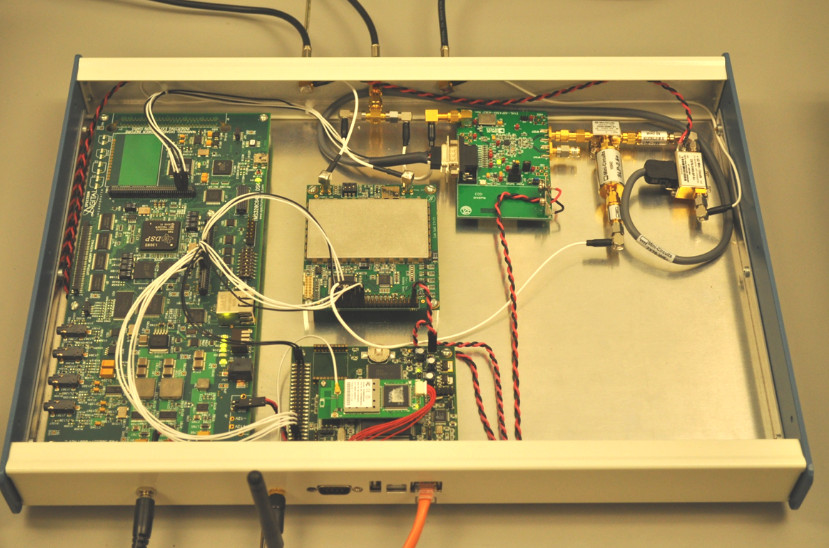
\includegraphics[scale=0.2]{pics/texas_spoofer.jpg}
    \caption{Civil GPS Spoofer}
  \end{figure}
  "The Civil GPS Spoofer"
  \begin{itemize}
    \item Laget et av et team fra \textit{The University of Texas at Austin} i 2012 \cite{EVPMUGA}
    \item Implementert i Software definert radio
    \item Simulere opptil 14 "falske" satellitter.
  \end{itemize}
\end{frame}

\begin{frame}
  \frametitle{"The Civil GPS Spoofer"}
  Nøkkelfunksjoner:
  \begin{itemize}
    \item Sømløs narring, offeret låser på en kopi av det autentiske signalet. Ingen forandring i løsning.
    \item Angriper manipulerer signalet.
    \item Angriperen har gjerne et stort spillerom under angrepet da oscillatoren i mottakeren ofte er av lav kvalitet.
  \end{itemize}
\end{frame}

\section{Deteksjon og mottiltak}
\begin{frame}
\frametitle{Deteksjon og mottiltak}
  \begin{itemize}
    \item Deteksjon
    \begin{itemize}
      \item Bruke flere GPS mottakere med kjent posisjon.
      \item Bruke stabil klokke som referanse.
    \end{itemize}
    \item Mottiltak: Bruke klokke som tidskilde.
  \end{itemize}
\end{frame}

\subsection{Flere GPS mottakere}
\begin{frame} 
  \frametitle{Flere GPS mottakere og kjent posisjon}
  \begin{itemize}
    \item En GPS mottakere med ukjent posisjon: Lett
    \item En GPS mottakere med kjent posisjon: Gjennomførbart
    \item To GPS mottakere med kjent posisjon: Svært komplisert
    \begin{itemize}
      \item Minimum en mottakere løser feil posisjon.
      \item Med mindre narren er like langt fra begge, forskjell i tidsløsning.  
    \end{itemize}
  \end{itemize}
  Kompleksiteten øker for hver GPS mottaker som legges til.
\end{frame}

\subsection{Referanseklokke}
\begin{frame}
  \frametitle{Referanseklokke}
  Med en stabil og pålitelig klokke, har en muligheter til å:
  \begin{itemize}
    \item Verifisere GPS løsning.
    \item Realisere nøyaktig timing selv når GPS disiplinering ikke er mulig.
  \end{itemize}
  \begin{columns}
    \column{0.5\textwidth}
      \begin{figure}
        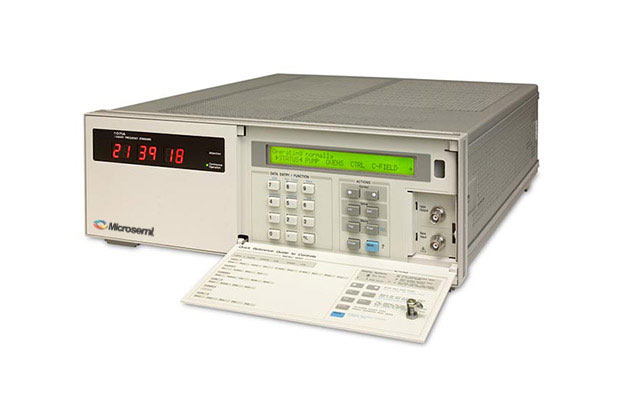
\includegraphics[scale=0.2]{pics/5071A.jpg}
        \caption{Symmetricom 5071A Cesium Primary Frequency Standard (500 000 NOK)}
      \end{figure}
    \column{0.5\textwidth}
      \begin{figure}
        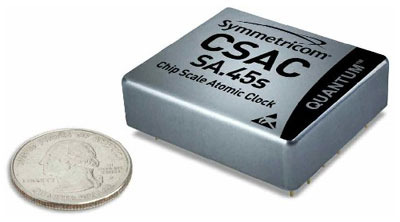
\includegraphics[scale=0.2]{thesis/graphics/csac.jpg}
      \caption{Symmetricom SA.45s CSAC (5000 NOK)}
    \end{figure}
  \end{columns}
\end{frame}

\begin{frame}
  \frametitle{Referanseklokke}
  Vi valgte Symmetricom SA.45s. 
  \begin{itemize}
    \item Lav vekt og størrelse
    \item Kortidsstabilitet på rundt ($10^{-11}$)
    \item Intern frekvensteller og styringsalgoritme
    \item Kommuniserer over RS-232
  \end{itemize}
\end{frame}

\section{Implementasjon}
\subsection{Krav}
\begin{frame}
  \frametitle{Krav}
  Følgende krav ble identifisert til systemet:
  \begin{itemize}
    \item Kunne detektere angrep hurtig
    \item Ha mulighet for å logge data
    \item Rask og enkel tilgang til innsamlet data
    \item Enkelt kunne koble til flere GPS mottakere
    \item Kunne administreres over nettverk
    \item Konfigurerbar 
  \end{itemize}
\end{frame}

\subsection{Sensor server arkitektur}
\begin{frame}
  \frametitle{Sensor server arkitektur}
  \begin{itemize}
    \item Mottaker + Raspberry PI = GPS mottaker med nettverkskort = Sensor
    \item Eliminerer behovet for lange signalkabler, mulig å bruke et vanlig nettverk:
    \begin{itemize}
      \item Fiber
      \item Mobilnett (3G og 4G)
      \item WiFi
    \end{itemize}
    \item Antall mottakere begrenset av serverens maskinvare.
  \end{itemize}
\end{frame}

\begin{frame}
  \frametitle{Sensor server arkitektur}
  \begin{itemize}
    \item 3000+ linjer med C99 kode
    \item Håndterer av/pålogging av klienter
    \item Håndtere mottak og formatering av GPS data
    \item En prosess per pålogging
    \item Delt minne mellom prosesser (anonym MMAP)
      \begin{itemize}
        \item Semaforer og barrierer for beskyttelse
      \end{itemize}
    \item Mulighet for brukere å koble på og gi kommandoer, f.eks:
      \begin{itemize}
        \item Rapporterer lokasjon og tid
        \item Rapportere server status
        \item Rapportere filterstatus
        \item Lagre og gjenopprette tilstand i sensorer
        \item Laste inn nye lokasjonsdata
        \item Avslutte egen og andres tilkobling
        \item Sende kommandoer til atomklokka 
      \end{itemize}
  \end{itemize}
\end{frame}

\subsubsection{Klokkemodell}
\begin{frame}
  \frametitle{Klokkemodell}
    Klokkemodellen brukt i oppgaven er designet av Harald Hauglin. Brukes til:
    \begin{itemize}
      \item Referanse for frekvensavvik og klokkedrift 
      \item Generere brukbare styringsparameter i tilfelle GPS løsning ikke lenger er til å stole på.
    \end{itemize}
    Modellen er logisk en del av serveren og kjører i en egen prosess.
    \begin{itemize}
      \item Kommuniserer kontinuerlig med atomklokka
      \item Blir regnet som "moden" etter to dager (konfigurerbart).
    \end{itemize}
\end{frame}

\subsubsection{Filtre}
\begin{frame}
  \frametitle{Filtre}
  Filtrene brukes til å detektere avvik. Enten:
        \begin{itemize}
          \item GPS basert
          \item Klokkemodell basert
        \end{itemize}
  For øyeblikket kun implementert tre filtre:
  \begin{itemize}
    \item Lokasjon og hastighetsfilter
                  \begin{itemize}
                    \item Data fra sensorene blir samlet formatert.
                    \item Sjekker løst posisjon og hastighet mot referanseverdier
                  \end{itemize}
    \item Fasehoppfilter
                    \begin{itemize}
                      \item Sammenlikner nåværende fase som rapportert av atomklokka med en pre-konfigurert grense.
                    \end{itemize}
    \item Frekvenskorreksjonsfilter
                    \begin{itemize}
                      \item Sammenlikner nåværende styringsverdi med en forventet styringsverdi regnet ut med modellen.
                    \end{itemize}
  \end{itemize}
  Pre-konfigurerte referanseverdier er basert på et gjennomsnitt kalkulert fra en lengre måleserie.
\end{frame}

\section{Lokasjon og hastighetsfilter test}
\begin{frame}
Det lå i planene å utføre en test med en ekte "spoofer". Dette hadde vi dessverre ikke tilgang til da vi utførte følgende test. Vi manipulerte derfor tidsløsningen ved å bevege antenne.
\frametitle{Oppsett}
  \begin{itemize}
    \item Server logger data fra klokka
    \item Sensorer logger data fra GPS
  \end{itemize}
  \subsection{Beskrivelse}
      \begin{figure}
        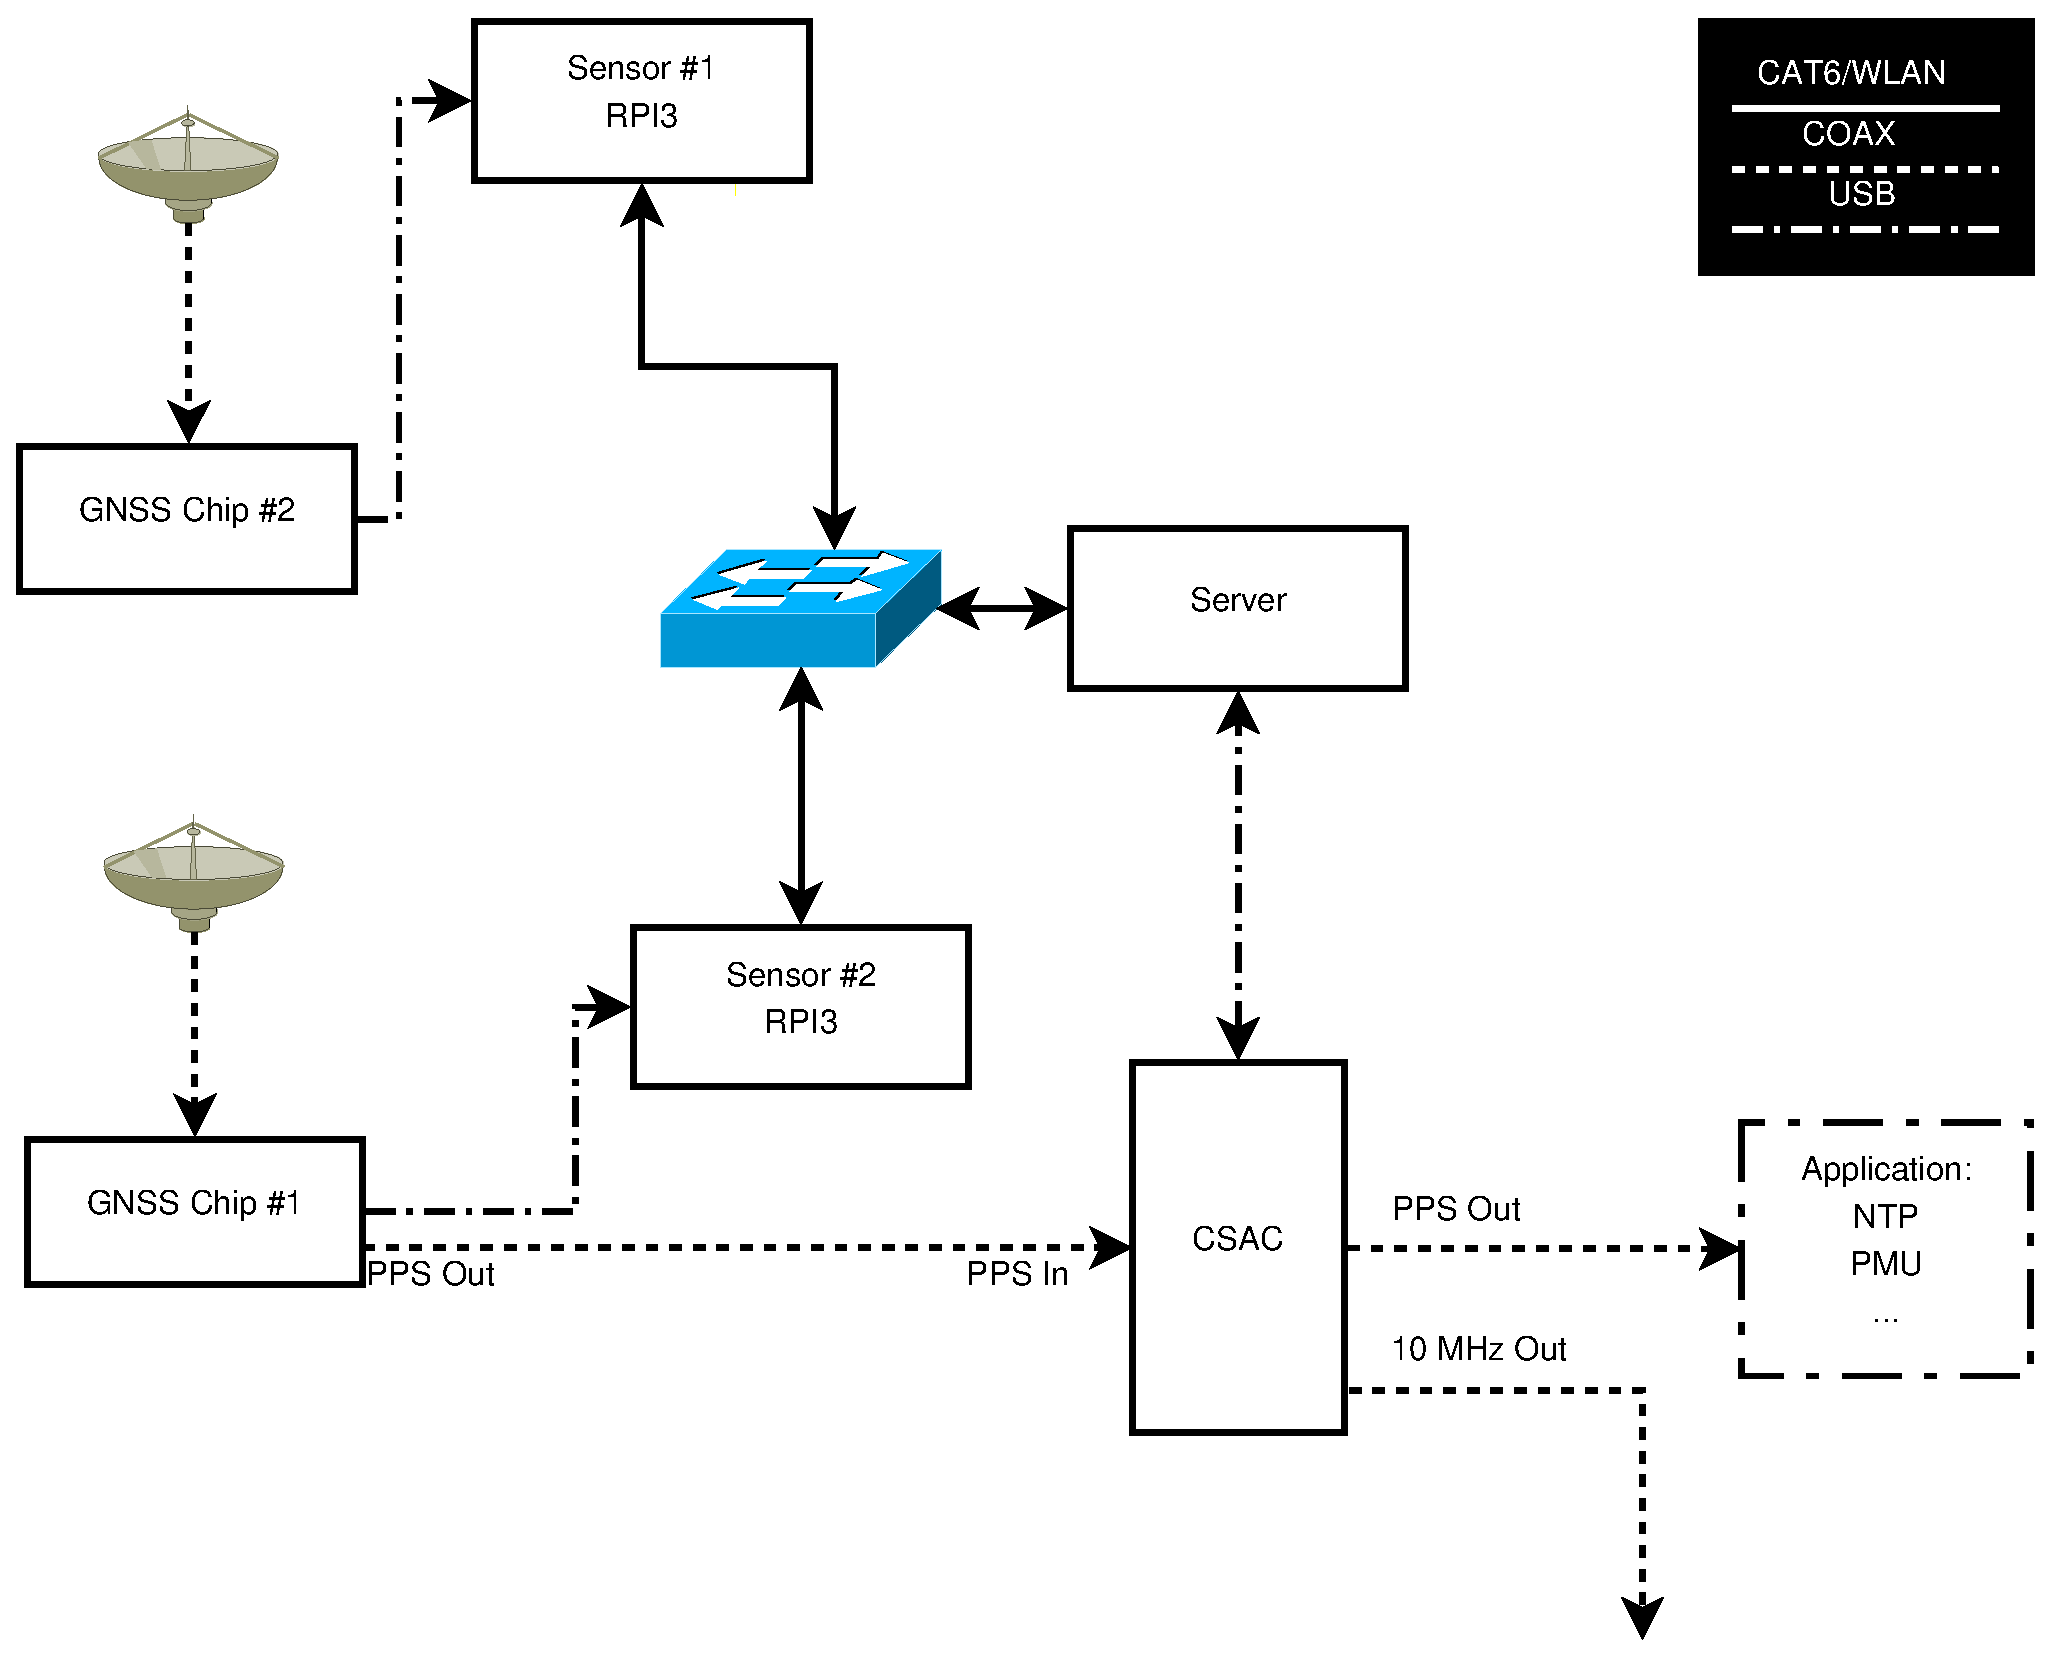
\includegraphics[scale=0.25]{thesis/graphics/server_layout.eps}
        \caption{Oppsett av server og klienter under test}
      \end{figure}
\end{frame}

\begin{frame}
\frametitle{Oppsett: måleutstyr}
  \begin{itemize}
    \item CNT-91 måler 1 PPS ut fra CSAC
    \item CNT-91 bruker 10 MHz fra tidslabb som referanse
  \end{itemize}
      \begin{figure}
        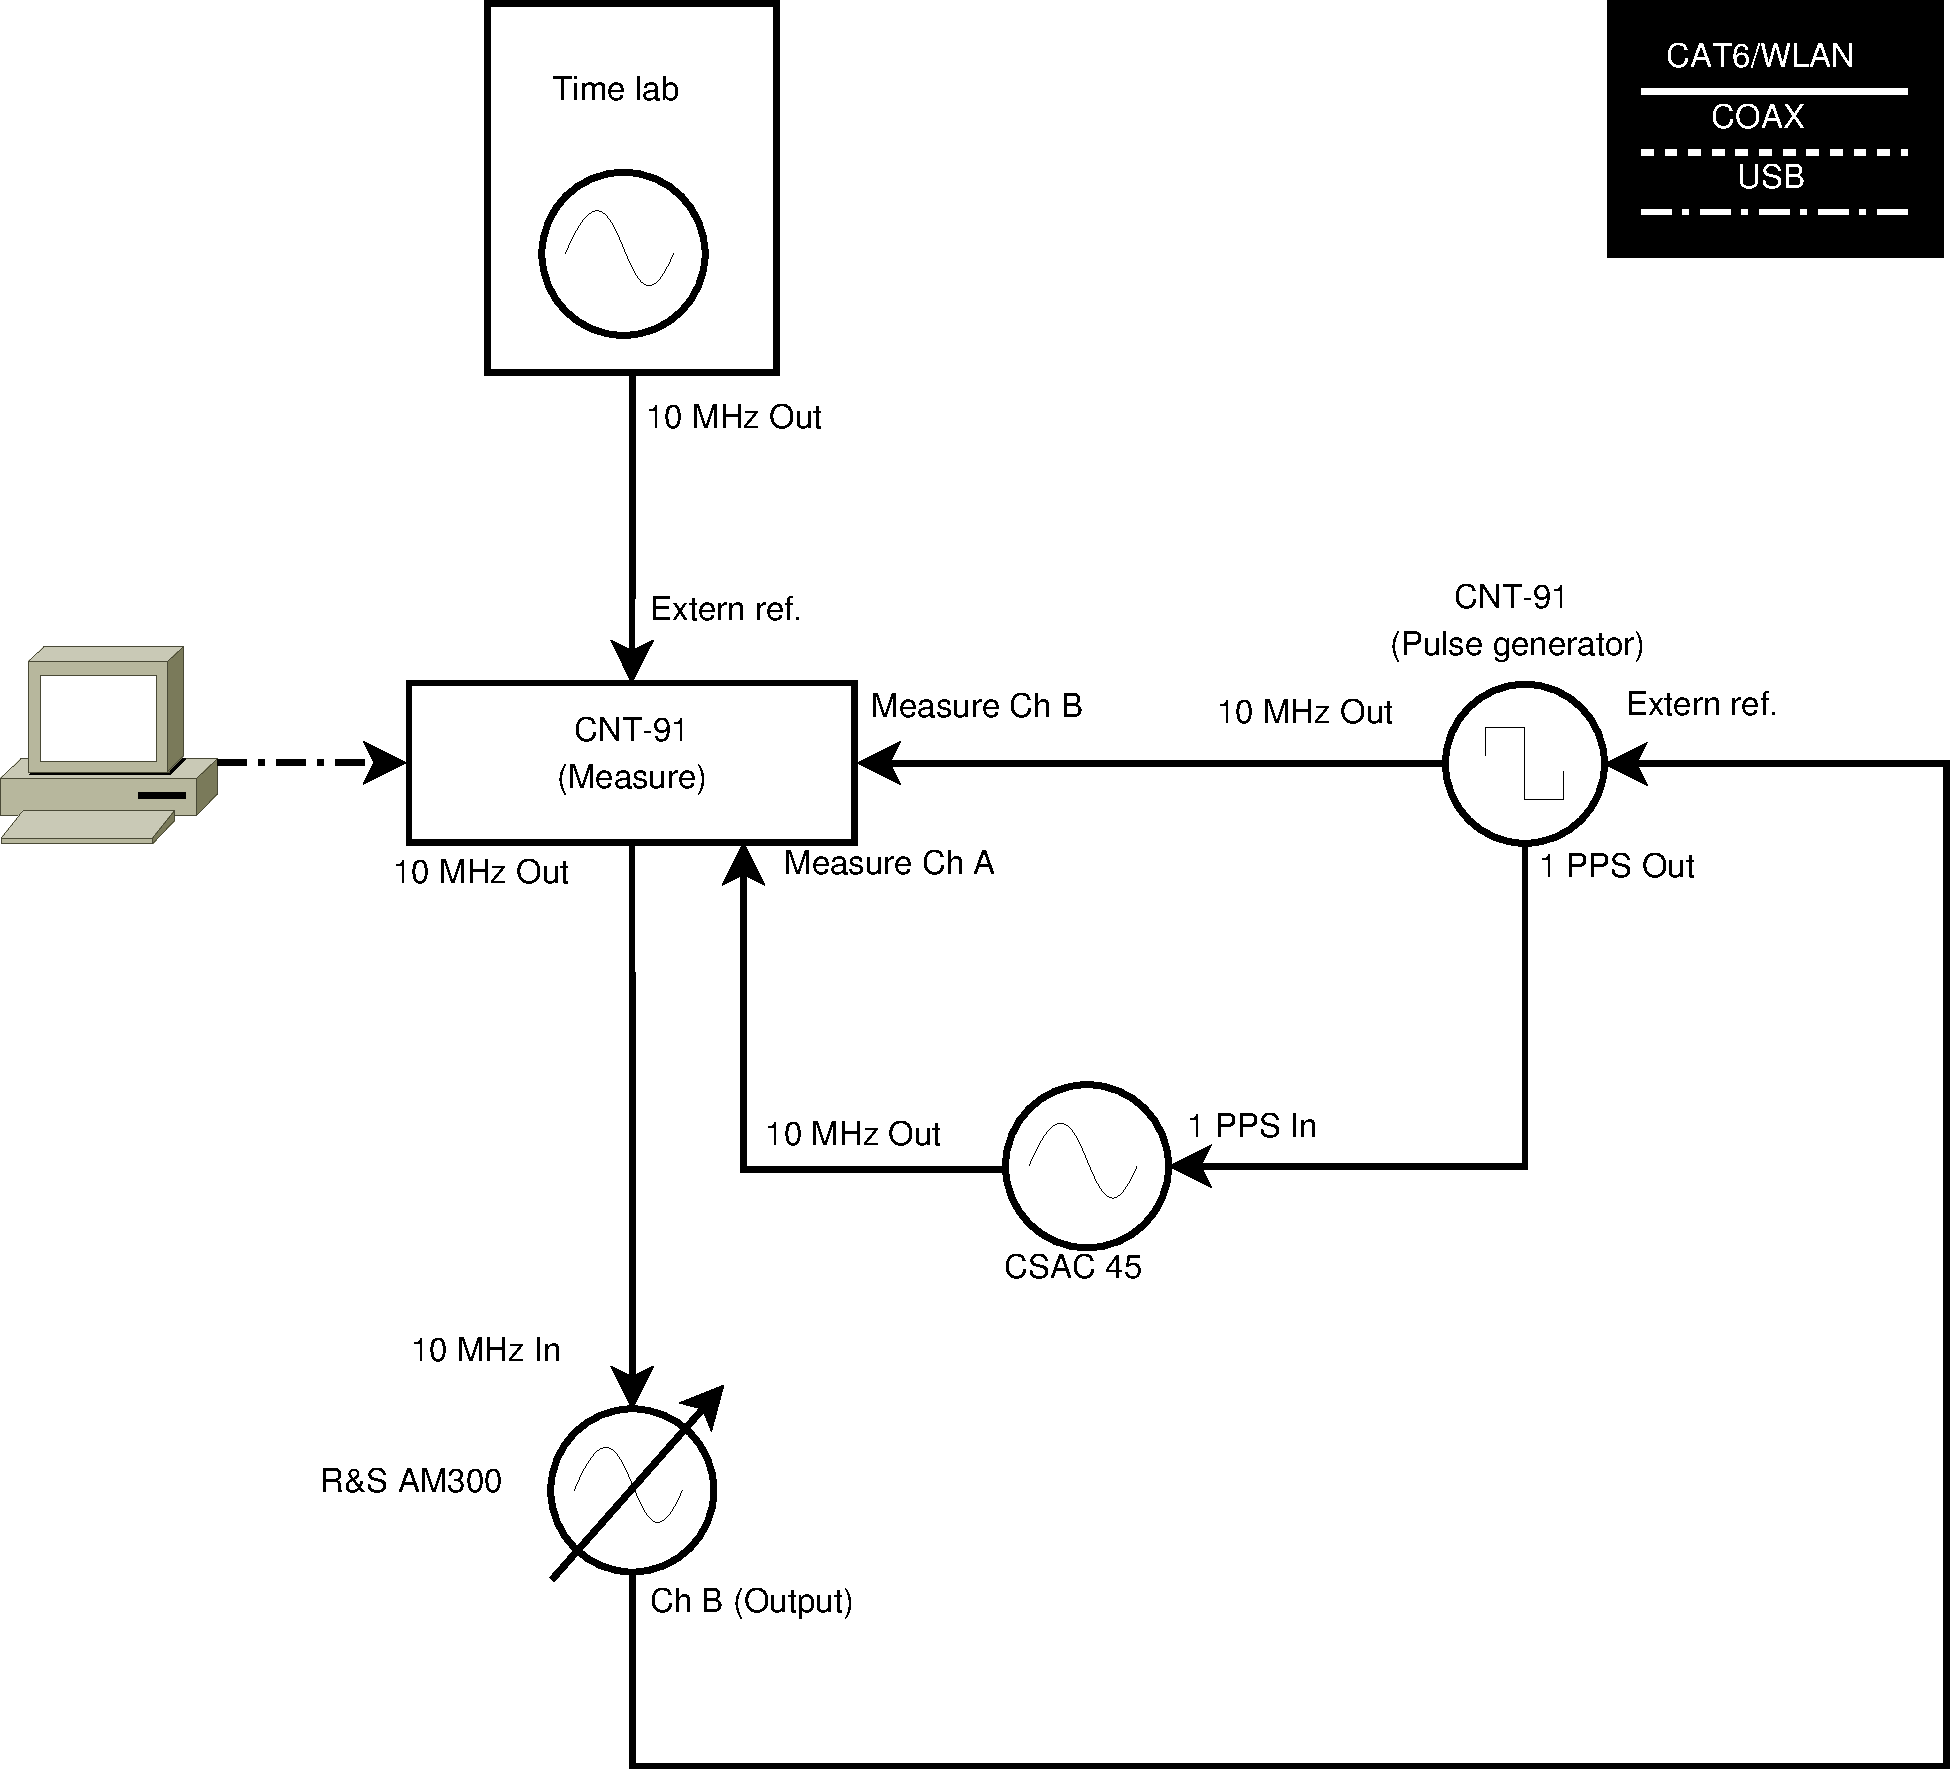
\includegraphics[scale=0.25]{thesis/graphics/measure_setup.pdf}
        \caption{Oppsett av måleutstyr}
      \end{figure}
\end{frame}

\begin{frame}
\frametitle{Oppsett: plassering av mottakere}
      \begin{figure}
        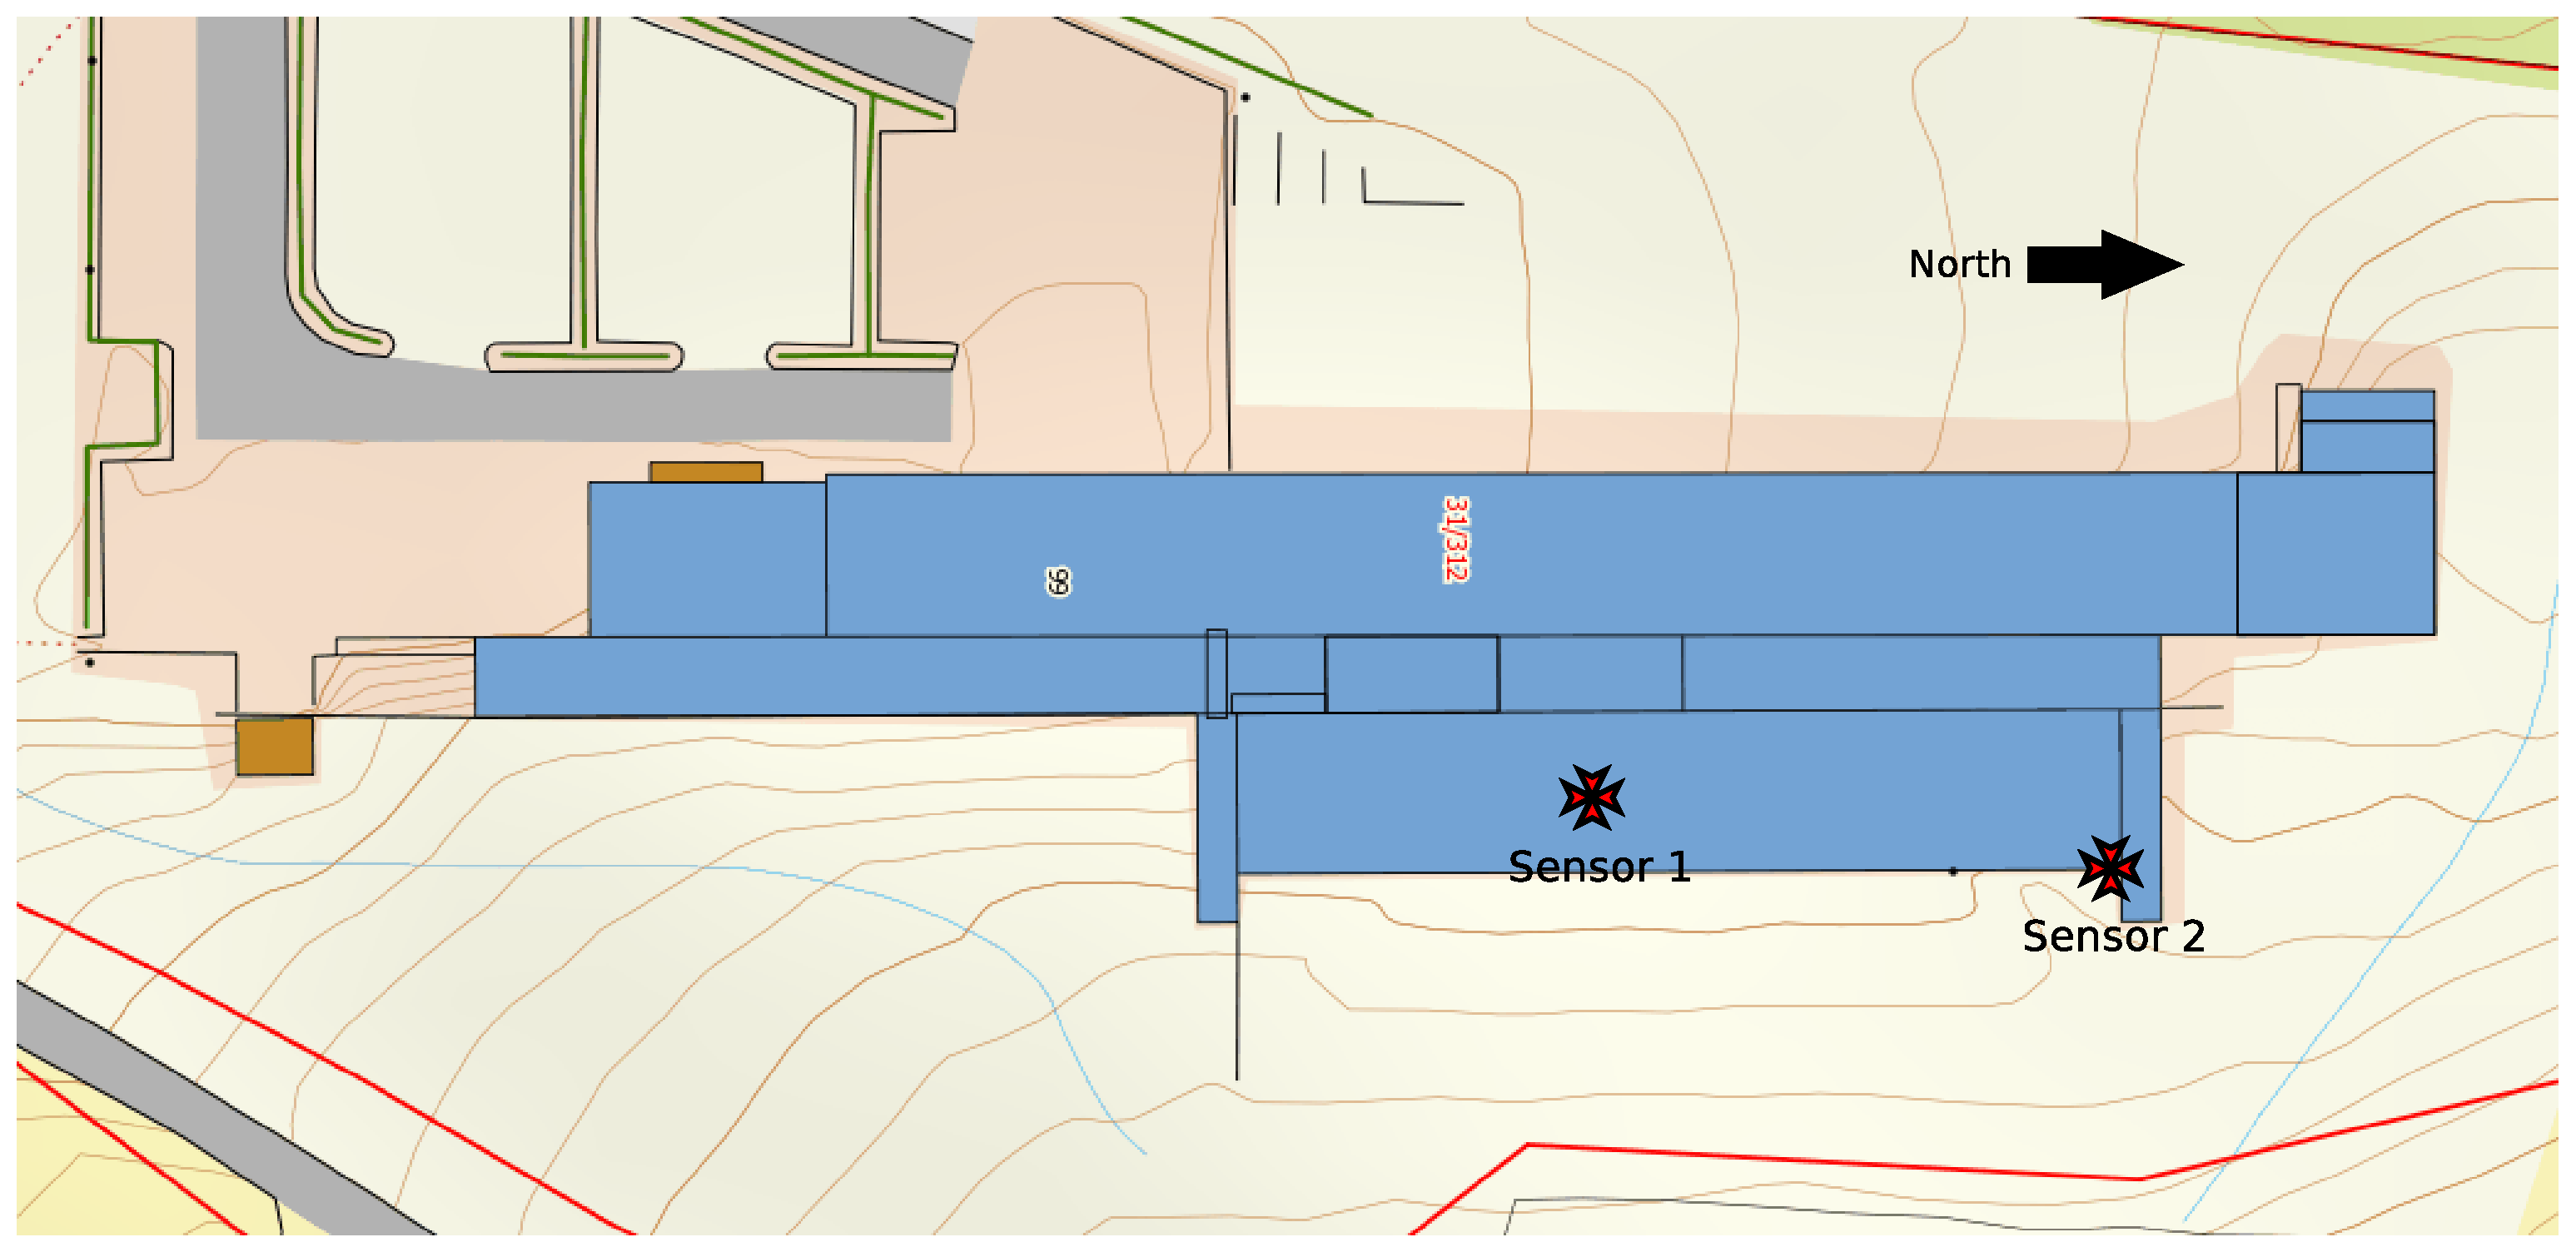
\includegraphics[scale=0.18]{thesis/graphics/roof.eps}
        \caption{Plasseringen av GPS mottakere}
      \end{figure}
\end{frame}

\begin{frame}
  \frametitle{Oppsett: grenseverdier for filter}
    \begin{table}[!htb]
      \centering
      \caption{Filter grenser}
      \label{gps_filter_table}
        \begin{tabular}{|l|l|l|}
        \hline
        \multicolumn{1}{|c|}{} & \multicolumn{1}{c|}{Sensor one} & \multicolumn{1}{c|}{Sensor two}         \\ \hline
        Høyde referanse                 & 123.8$^{\circ}$ & 122.427$^{\circ}$                            \\ \hline
        Lengdegrad referanse                & 1102.1948$^{\circ}$ & 1102.1934$^{\circ}$                     \\ \hline
        Breddegrad referanse                 & 5958.5448$^{\circ}$ & 5958.5231$^{\circ}$                     \\ \hline
        Hastighet referanse                    & 0 knot        & 0 knot                                       \\ \hline
        Høyde avvik                 & 10$^{\circ}$        & 10$^{\circ}$                            \\ \hline
        Lengdegrad avvik                & 0.005$^{\circ}$     & 0.005$^{\circ}$                         \\ \hline
        Breddegrad avvik                 & 0.005$^{\circ}$     & 0.005$^{\circ}$                         \\ \hline
        Hastighet avvik                    & 10 knot        & 10 knot                                     \\ \hline
        \end{tabular}
    \end{table}
\end{frame}

\begin{frame}
\frametitle{Utførelse}
Sekund 0 er 10:48.
      \begin{itemize}
        \item 10:58 - 600s: Beveget antenne 1 mot antenne 2
        \item 11:07 - 1140s: Beveget antenne 2 mot antenne 1
        \item 11:12 - 1560s: Viftet antenne 1 rundt i en halvsirkel
        \item 11:18 - 1800s: Viftet antenne 2 rundt i en halvsirkel
        \item 11:20 - 1920s: Dekket antenne 1 med aluminiumsfolie
        \item 11:25 - 2220s: Dekket antenne 2 med aluminiumsfolie
      \end{itemize}
\end{frame}

\begin{frame}
\frametitle{Utførelse}
\begin{center}
\begin{tikzpicture}
  \node (img1) {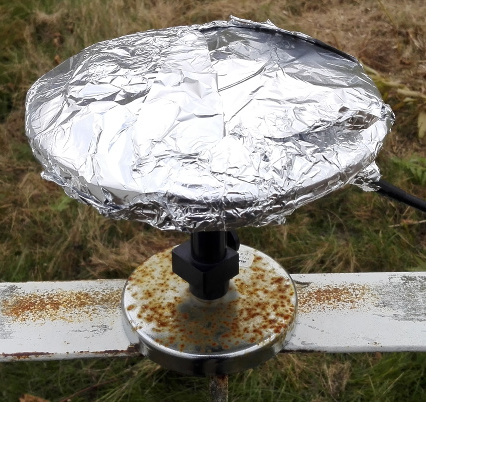
\includegraphics[height=5cm]{thesis/graphics/antenna_foil_over_hacked.jpg}};
  \node (img2) at (img1.south east) {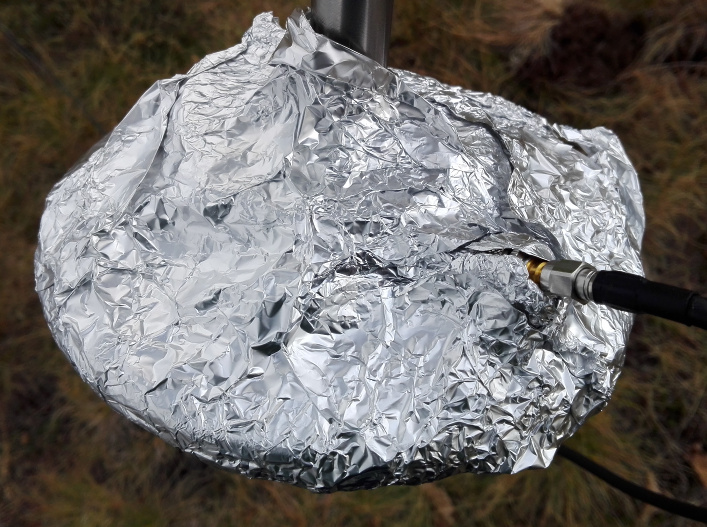
\includegraphics[height=4.5cm]{thesis/graphics/antenna_foil_cover.jpg}};
\end{tikzpicture}
\end{center}
\end{frame}

\begin{frame}[fragile]
\frametitle{Observasjon: Server log}
Utdrag fra server log:
      \begin{lstlisting}[basicstyle=\ttfamily\tiny]
        [10/10/16 - 10:59:17] [ ALARM ] Sensor 1 triggered LS filter!
        [10/10/16 - 11:04:35] [ ALARM ] Sensor 1 cleared LS filter!
        [10/10/16 - 11:08:27] [ ALARM ] Sensor 2 triggered LS filter!
        [10/10/16 - 11:13:43] [ ALARM ] Sensor 2 cleared LS filter!
        [10/10/16 - 11:22:03] [ ALARM ] Sensor 1 triggered LS filter!
        [10/10/16 - 11:29:21] [ ALARM ] Sensor 1 cleared LS filter!
        [10/10/16 - 11:27:31] [ ALARM ] Sensor 2 triggered LS filter!
        [10/10/16 - 11:34:16] [ ALARM ] Sensor 2 cleared LS filter!
        [10/10/16 - 11:34:17] [ ALARM ] Sensor 2 triggered LS filter!
        [10/10/16 - 11:34:20] [ ALARM ] Sensor 2 cleared LS filter!
      \end{lstlisting} 
\begin{itemize}
  \item Ingen falske positive.
  \item Hastighetsfilteret ble ikke utløst
\end{itemize}
\end{frame}

\begin{frame}
\frametitle{Observasjon: GPS log Sensor 1}
  \subsection{Observasjon}
    \vspace{-40pt}
    \begin{columns}
      \column{0.5\textwidth}
      \begin{figure}
        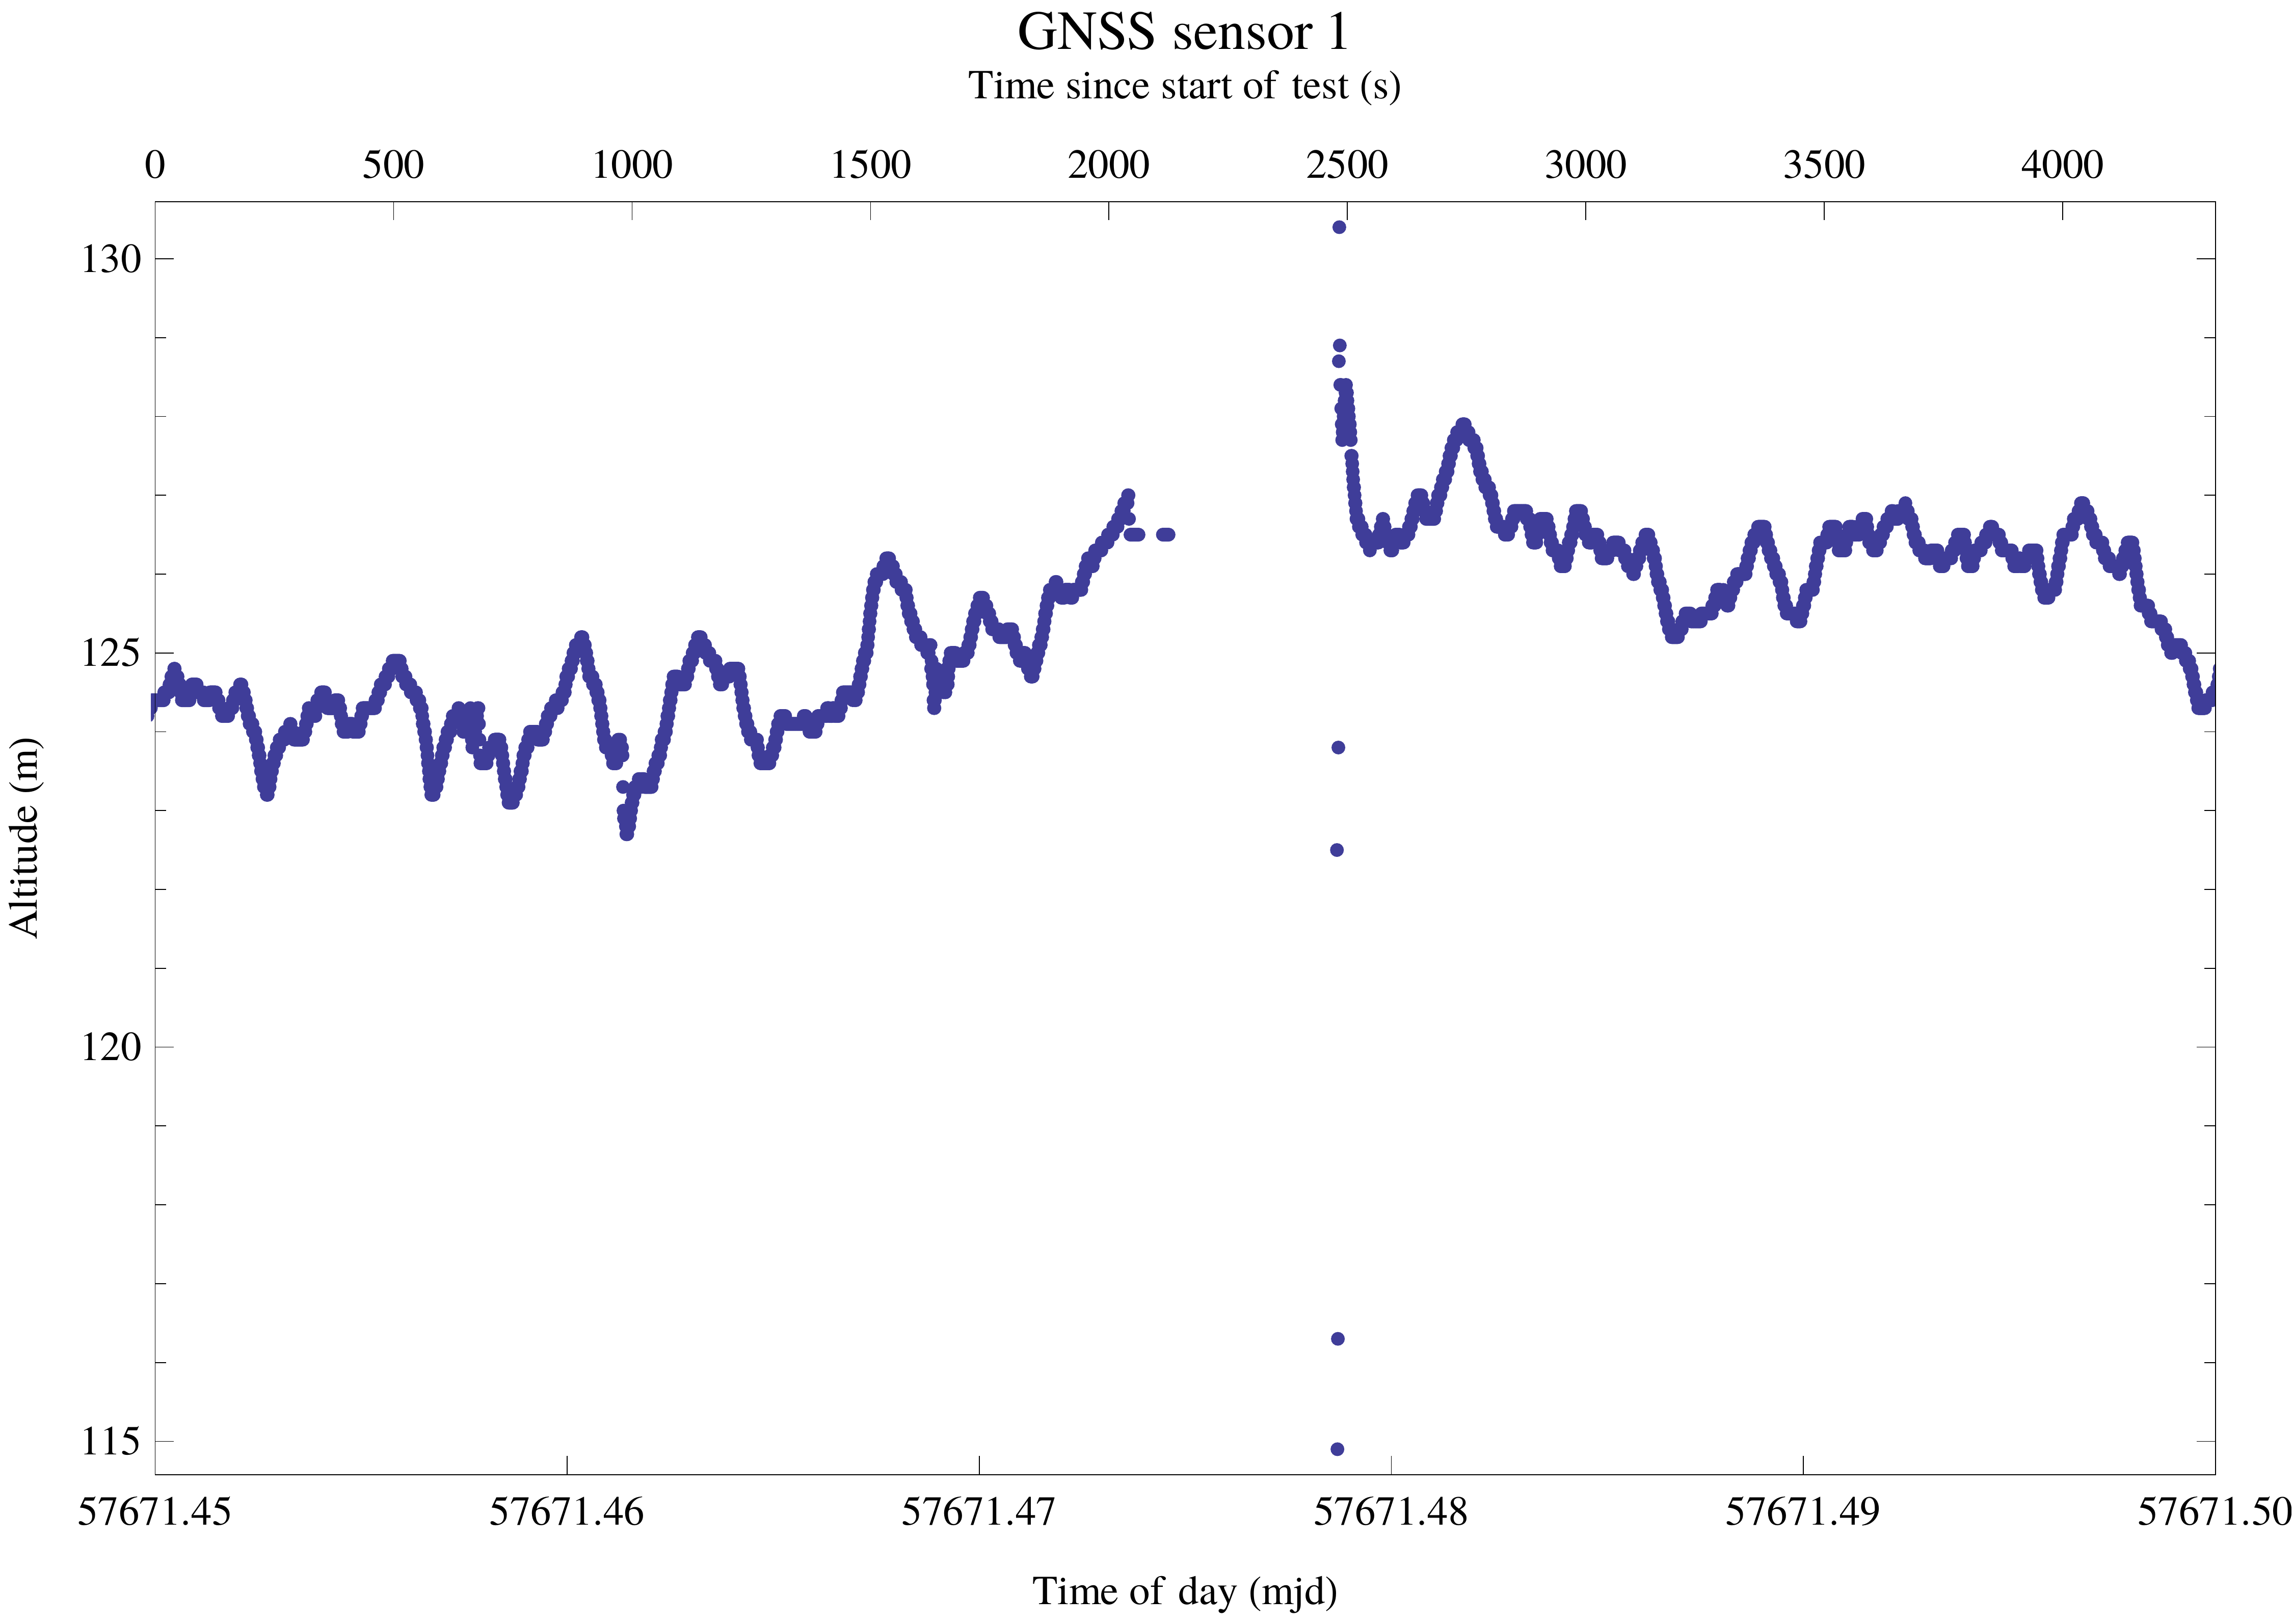
\includegraphics[scale=0.40]{thesis/graphics/gnssAlt1-1.png}
      \end{figure}
      \vspace{-30pt}
      \begin{figure}
        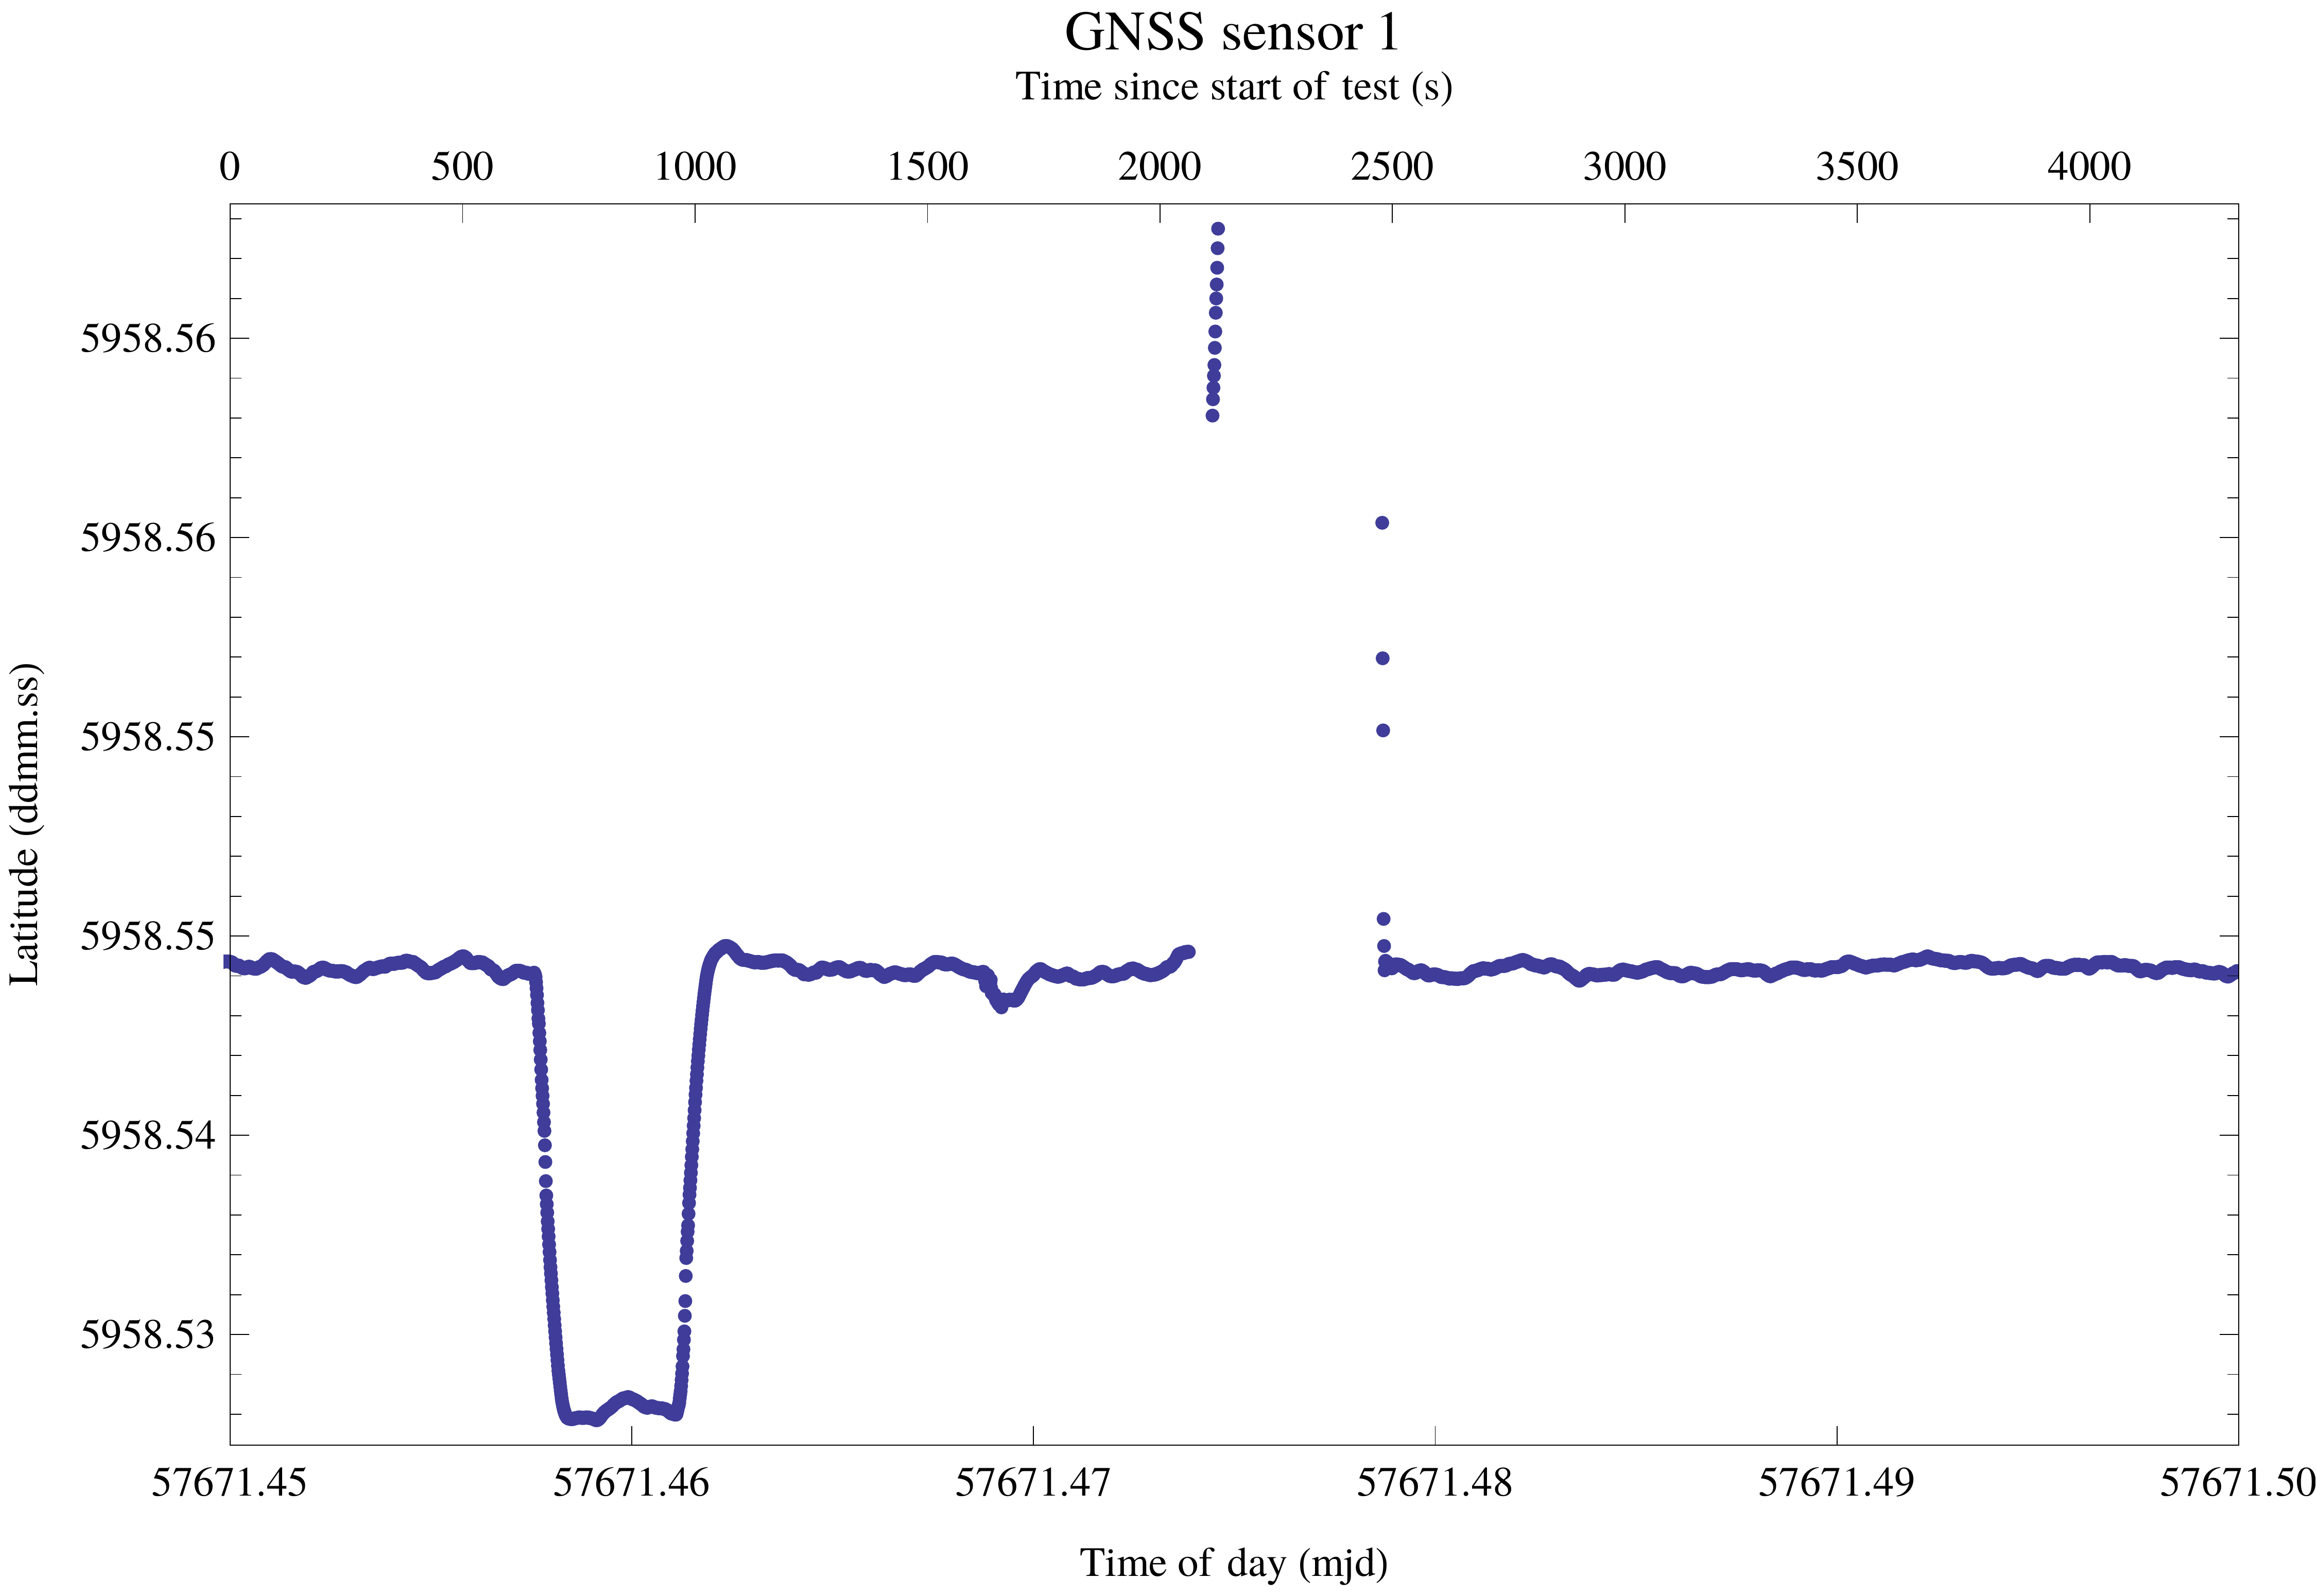
\includegraphics[scale=0.40]{thesis/graphics/gnssLat1-1.png}
      \end{figure}
      \column{0.5\textwidth}
      \begin{figure}
        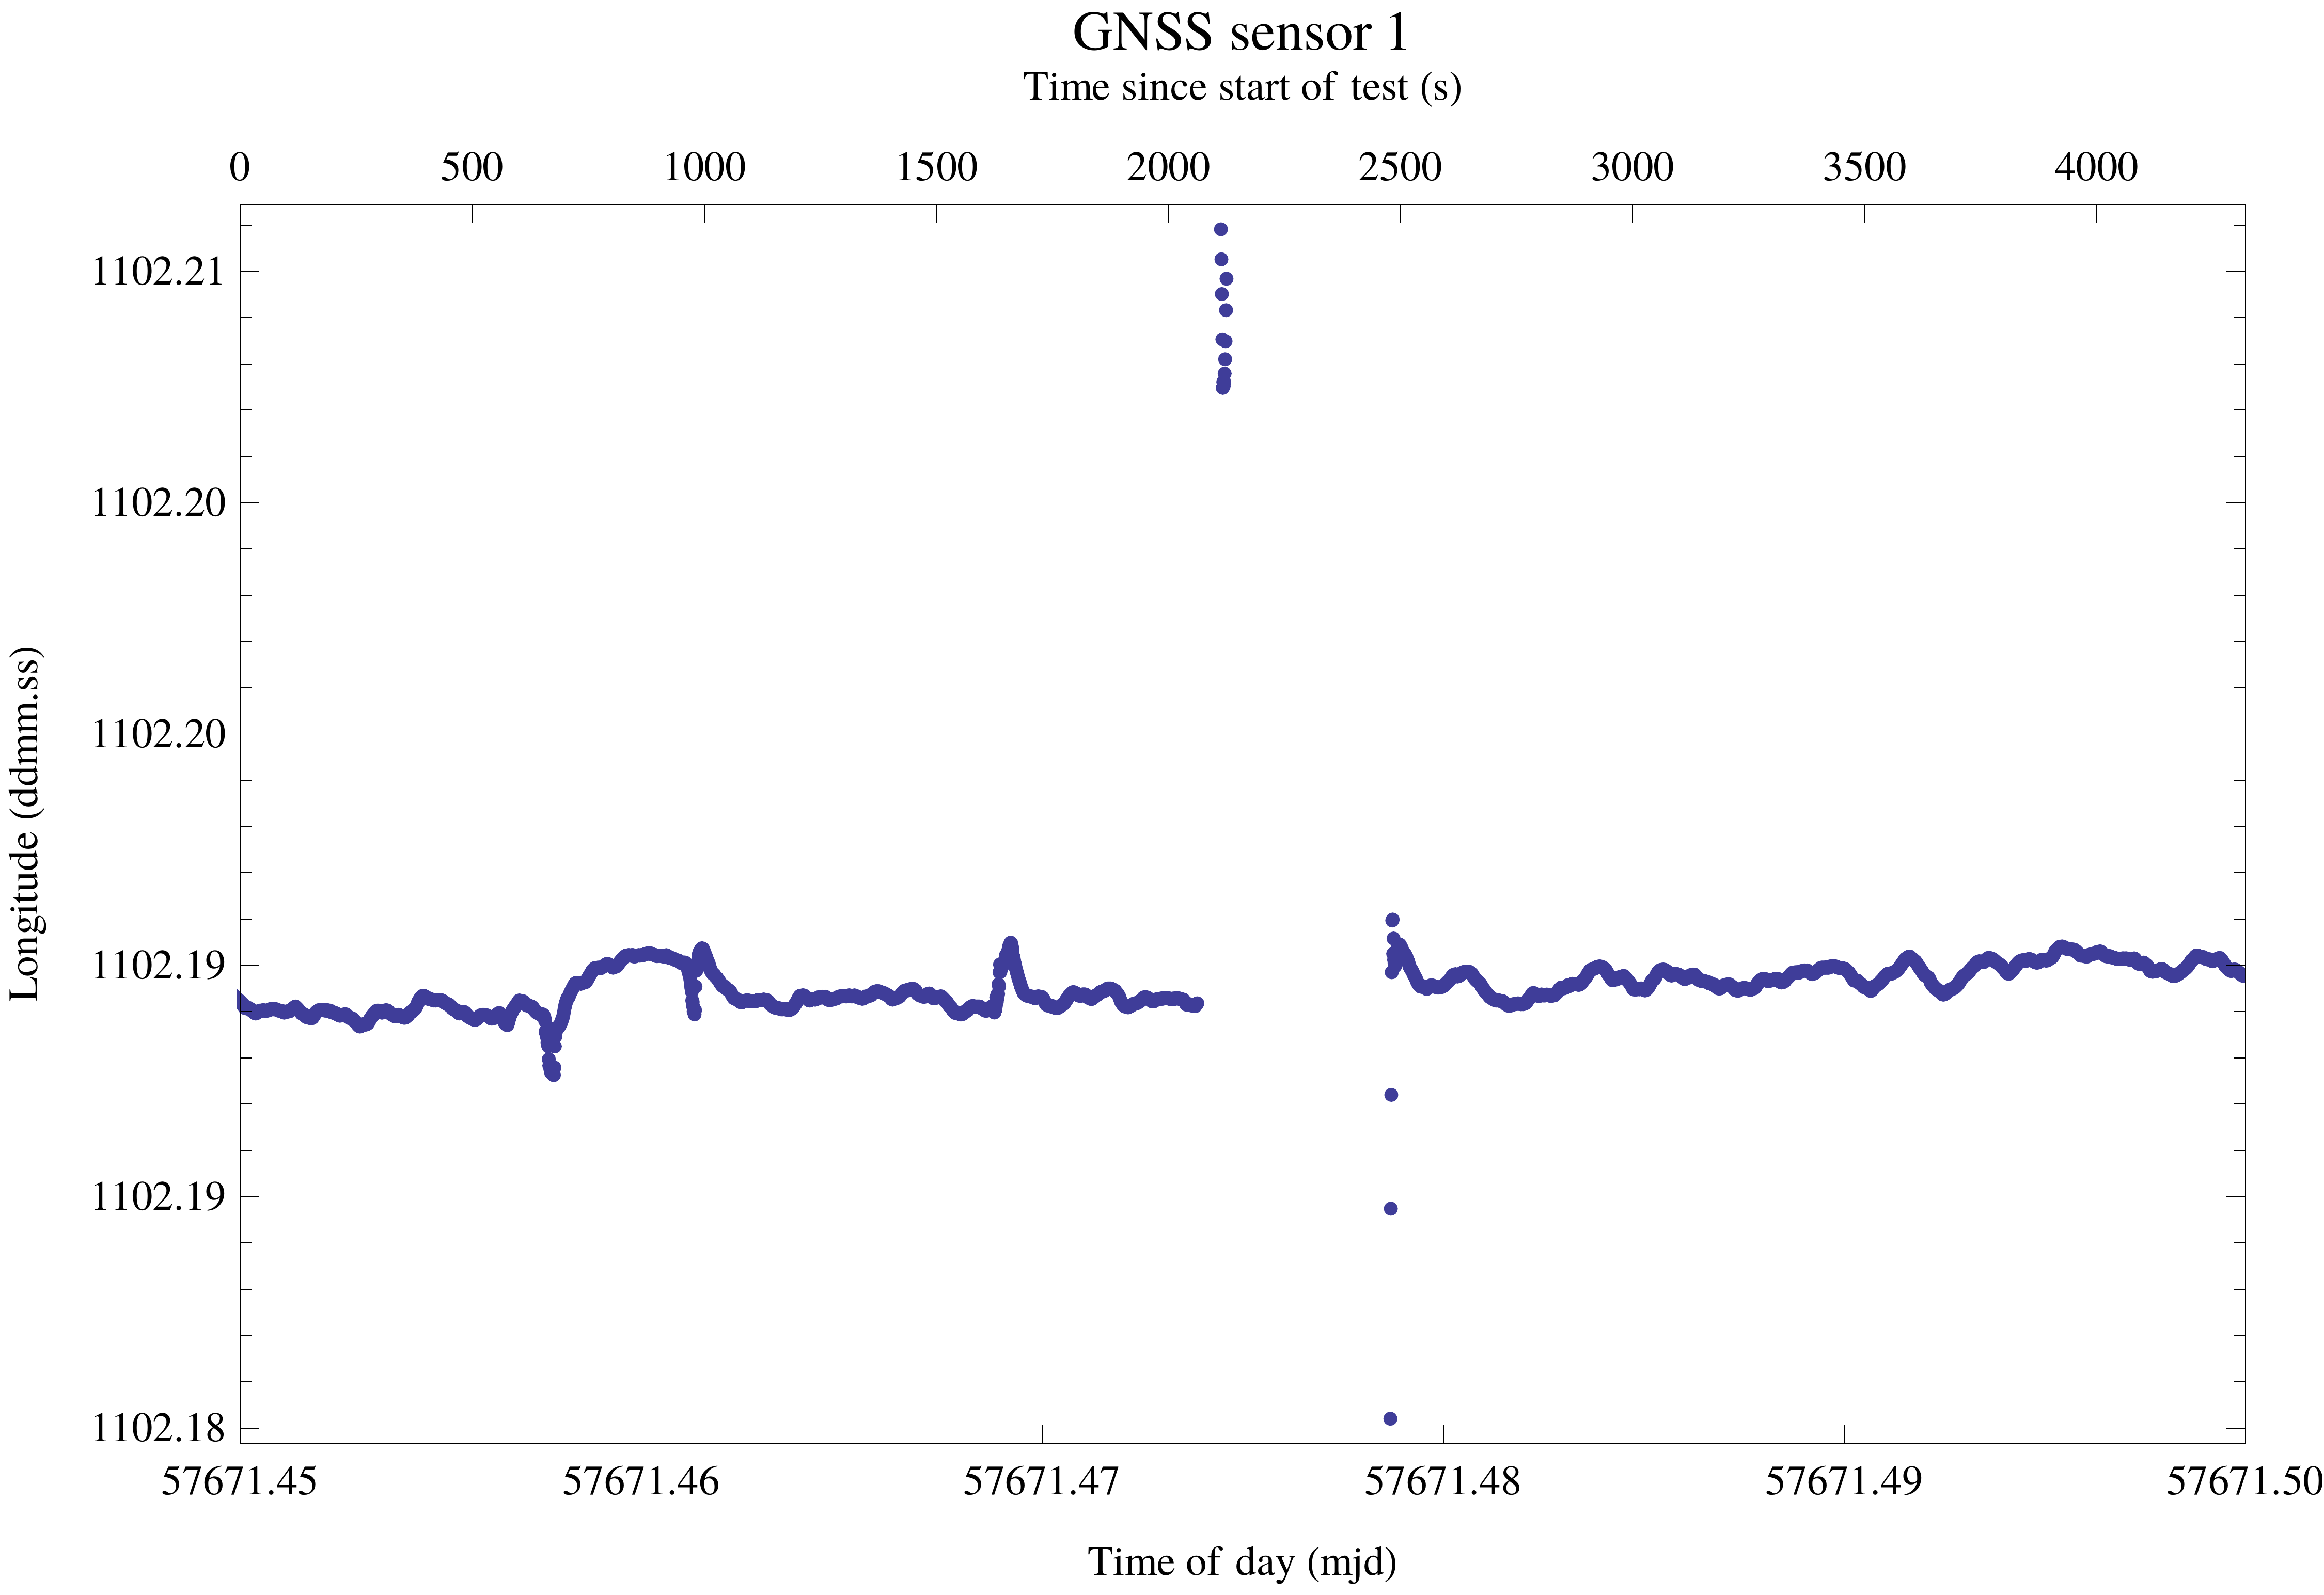
\includegraphics[scale=0.40]{thesis/graphics/gnssLong1-1.png}
      \end{figure}
      \vspace{-30pt}
      \begin{figure}
        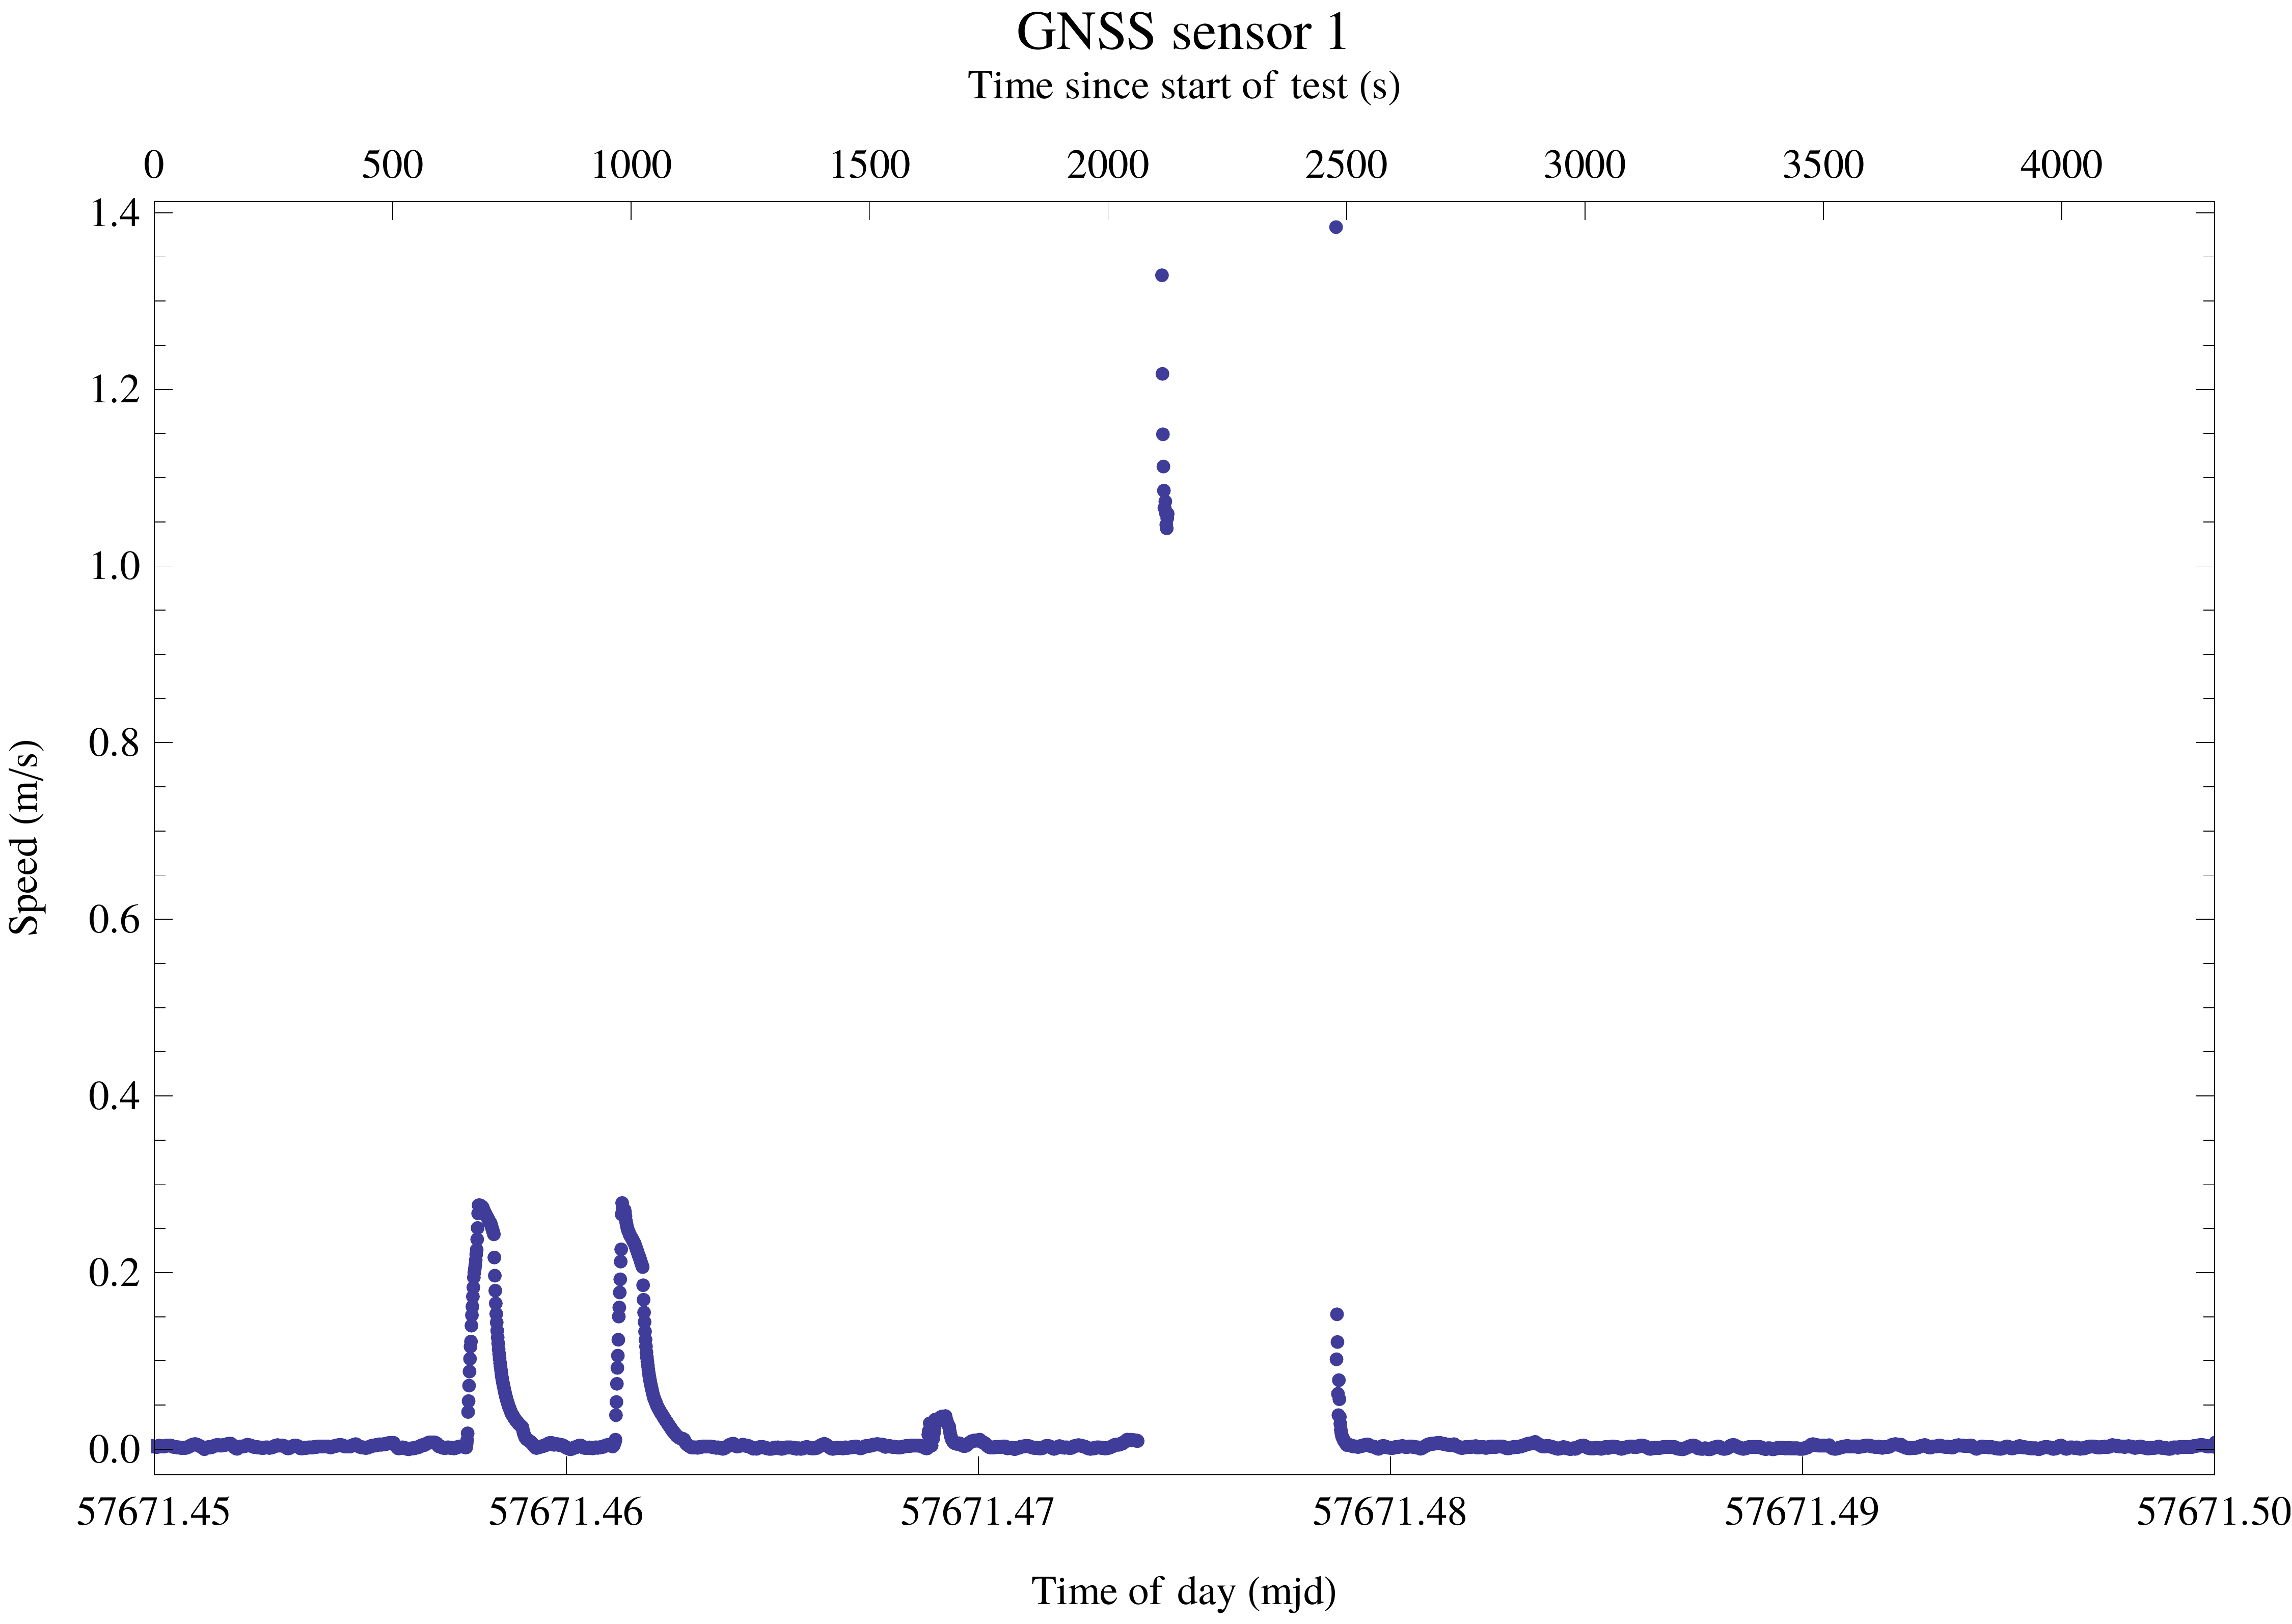
\includegraphics[scale=0.40]{thesis/graphics/gnssSpeed1-1.png}
      \end{figure}
    \end{columns}  
\end{frame}

\begin{frame}
\frametitle{Observasjon: GPS log Sensor 2}
    \vspace{-40pt}
    \begin{columns}
      \column{0.5\textwidth}
      \begin{figure}
        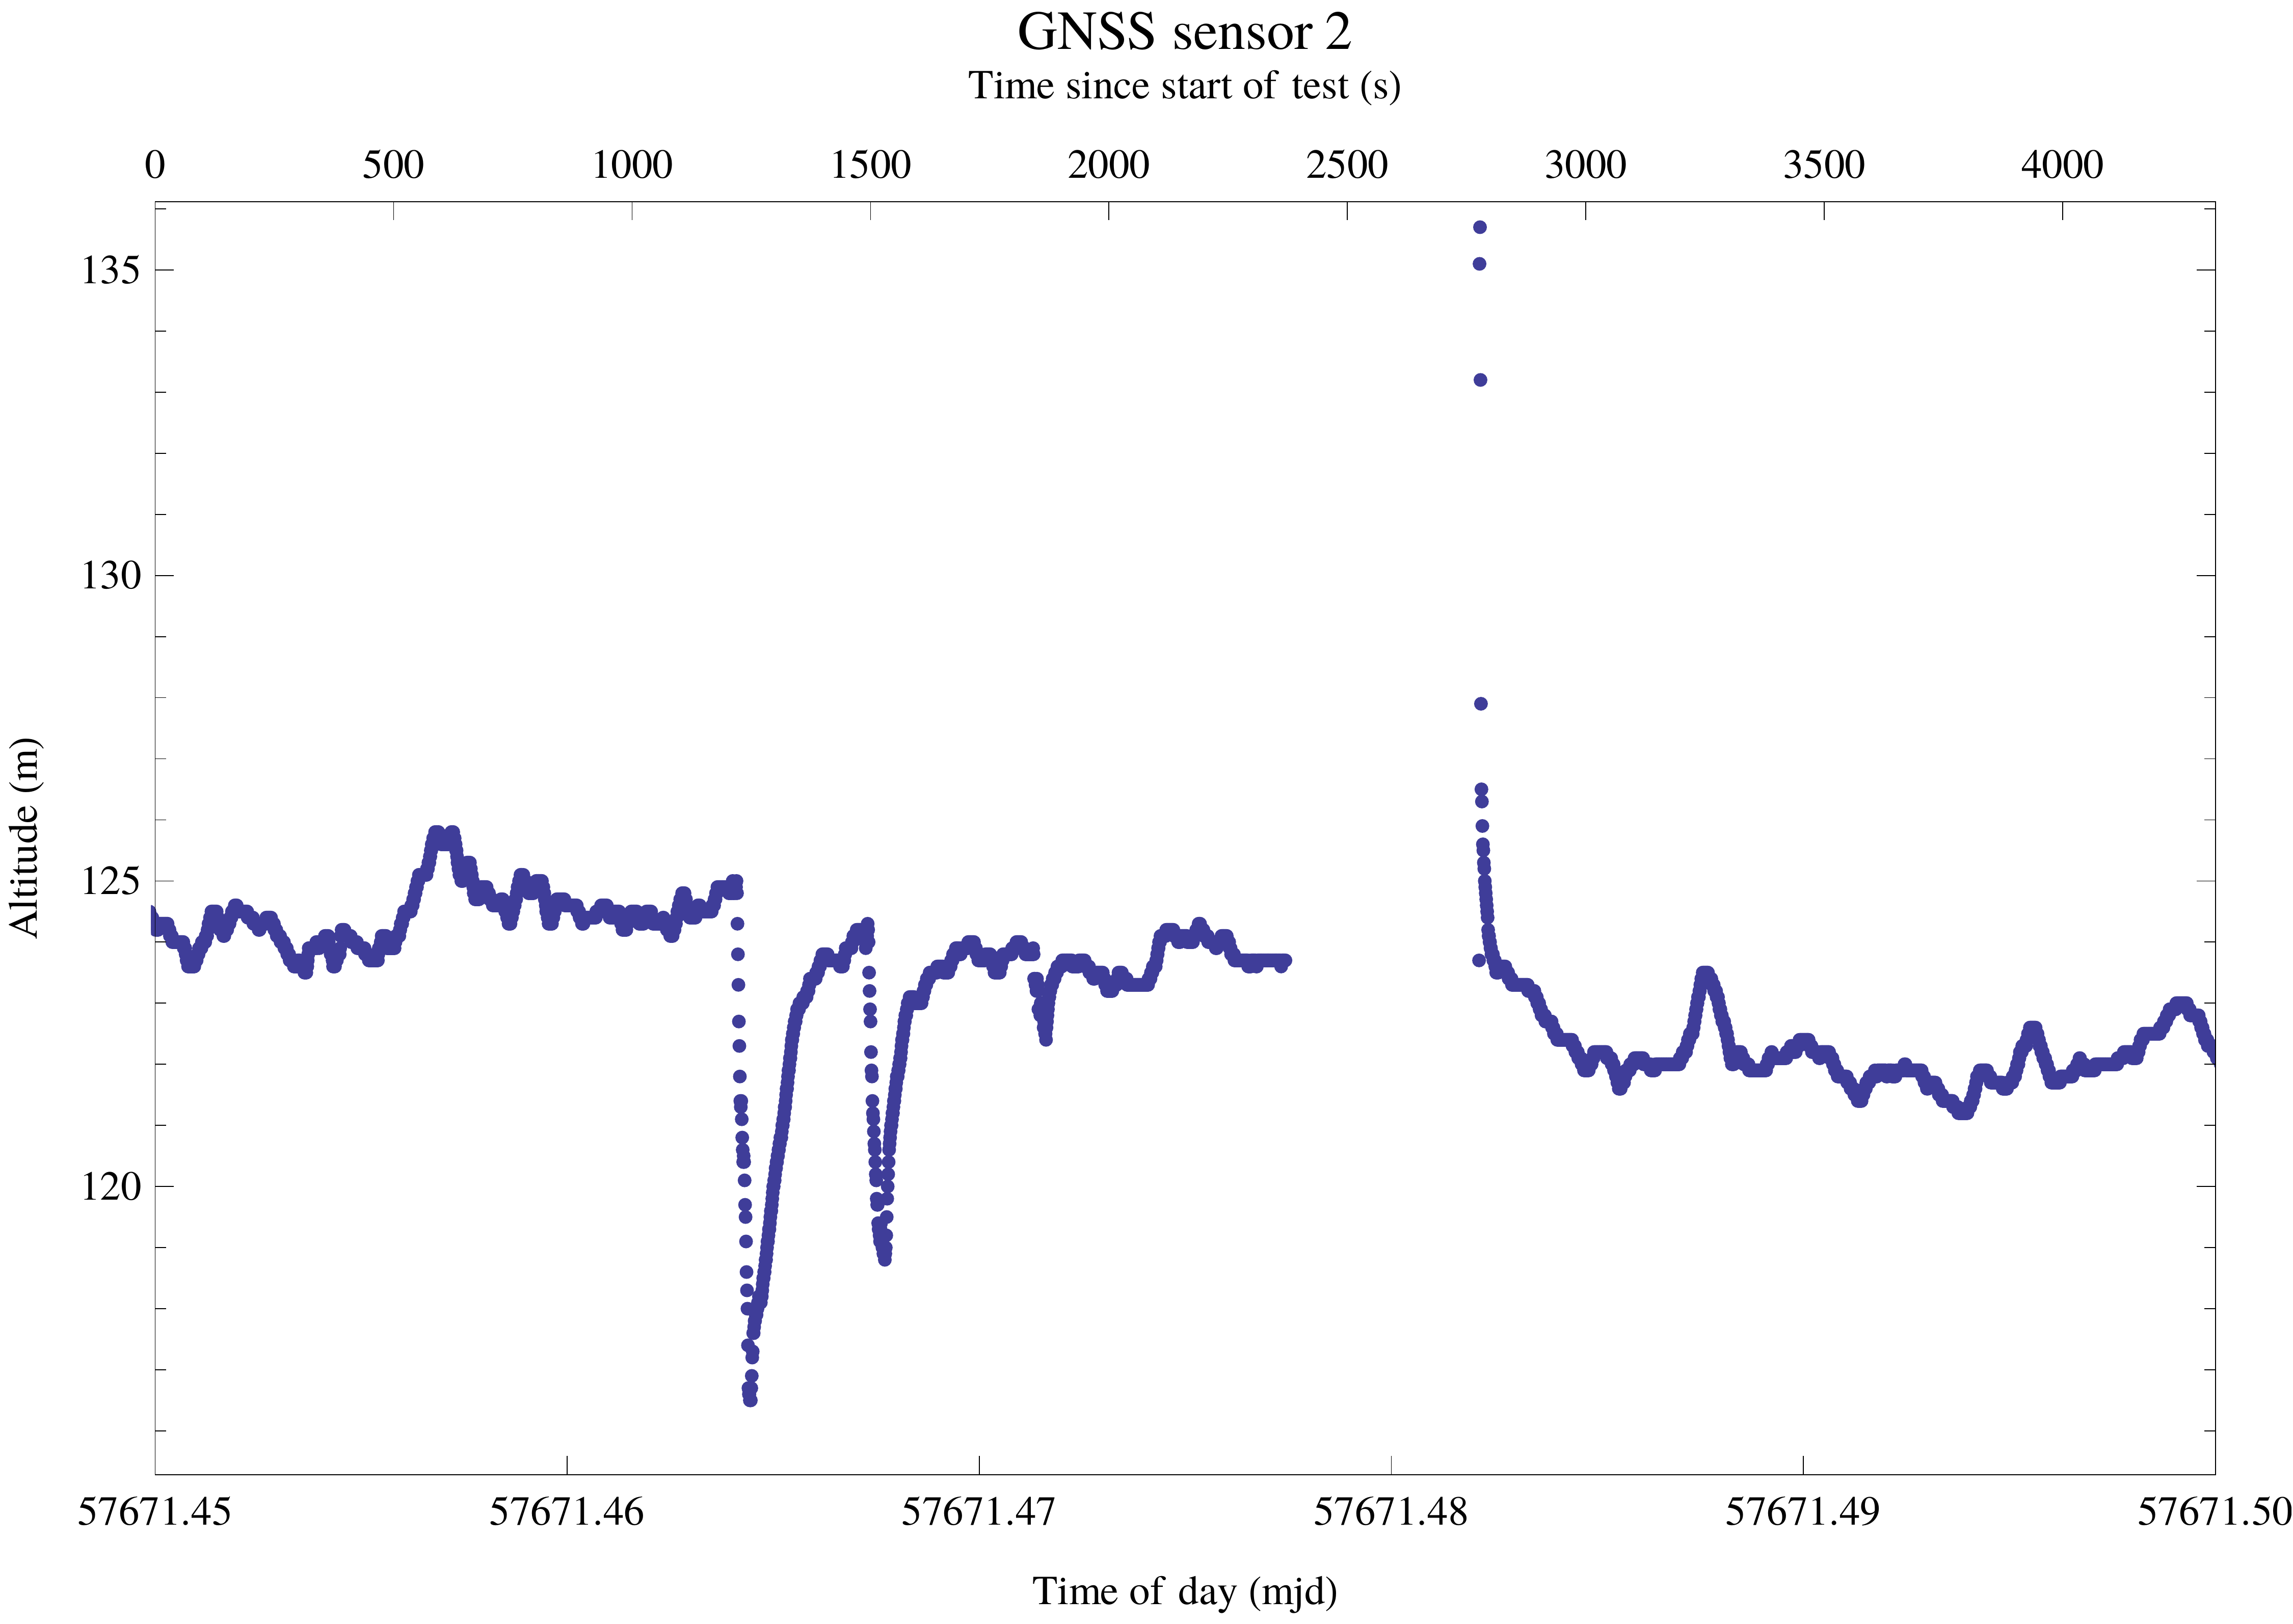
\includegraphics[scale=0.40]{thesis/graphics/gnssAlt2-1.png}
      \end{figure}
      \vspace{-30pt}
      \begin{figure}
        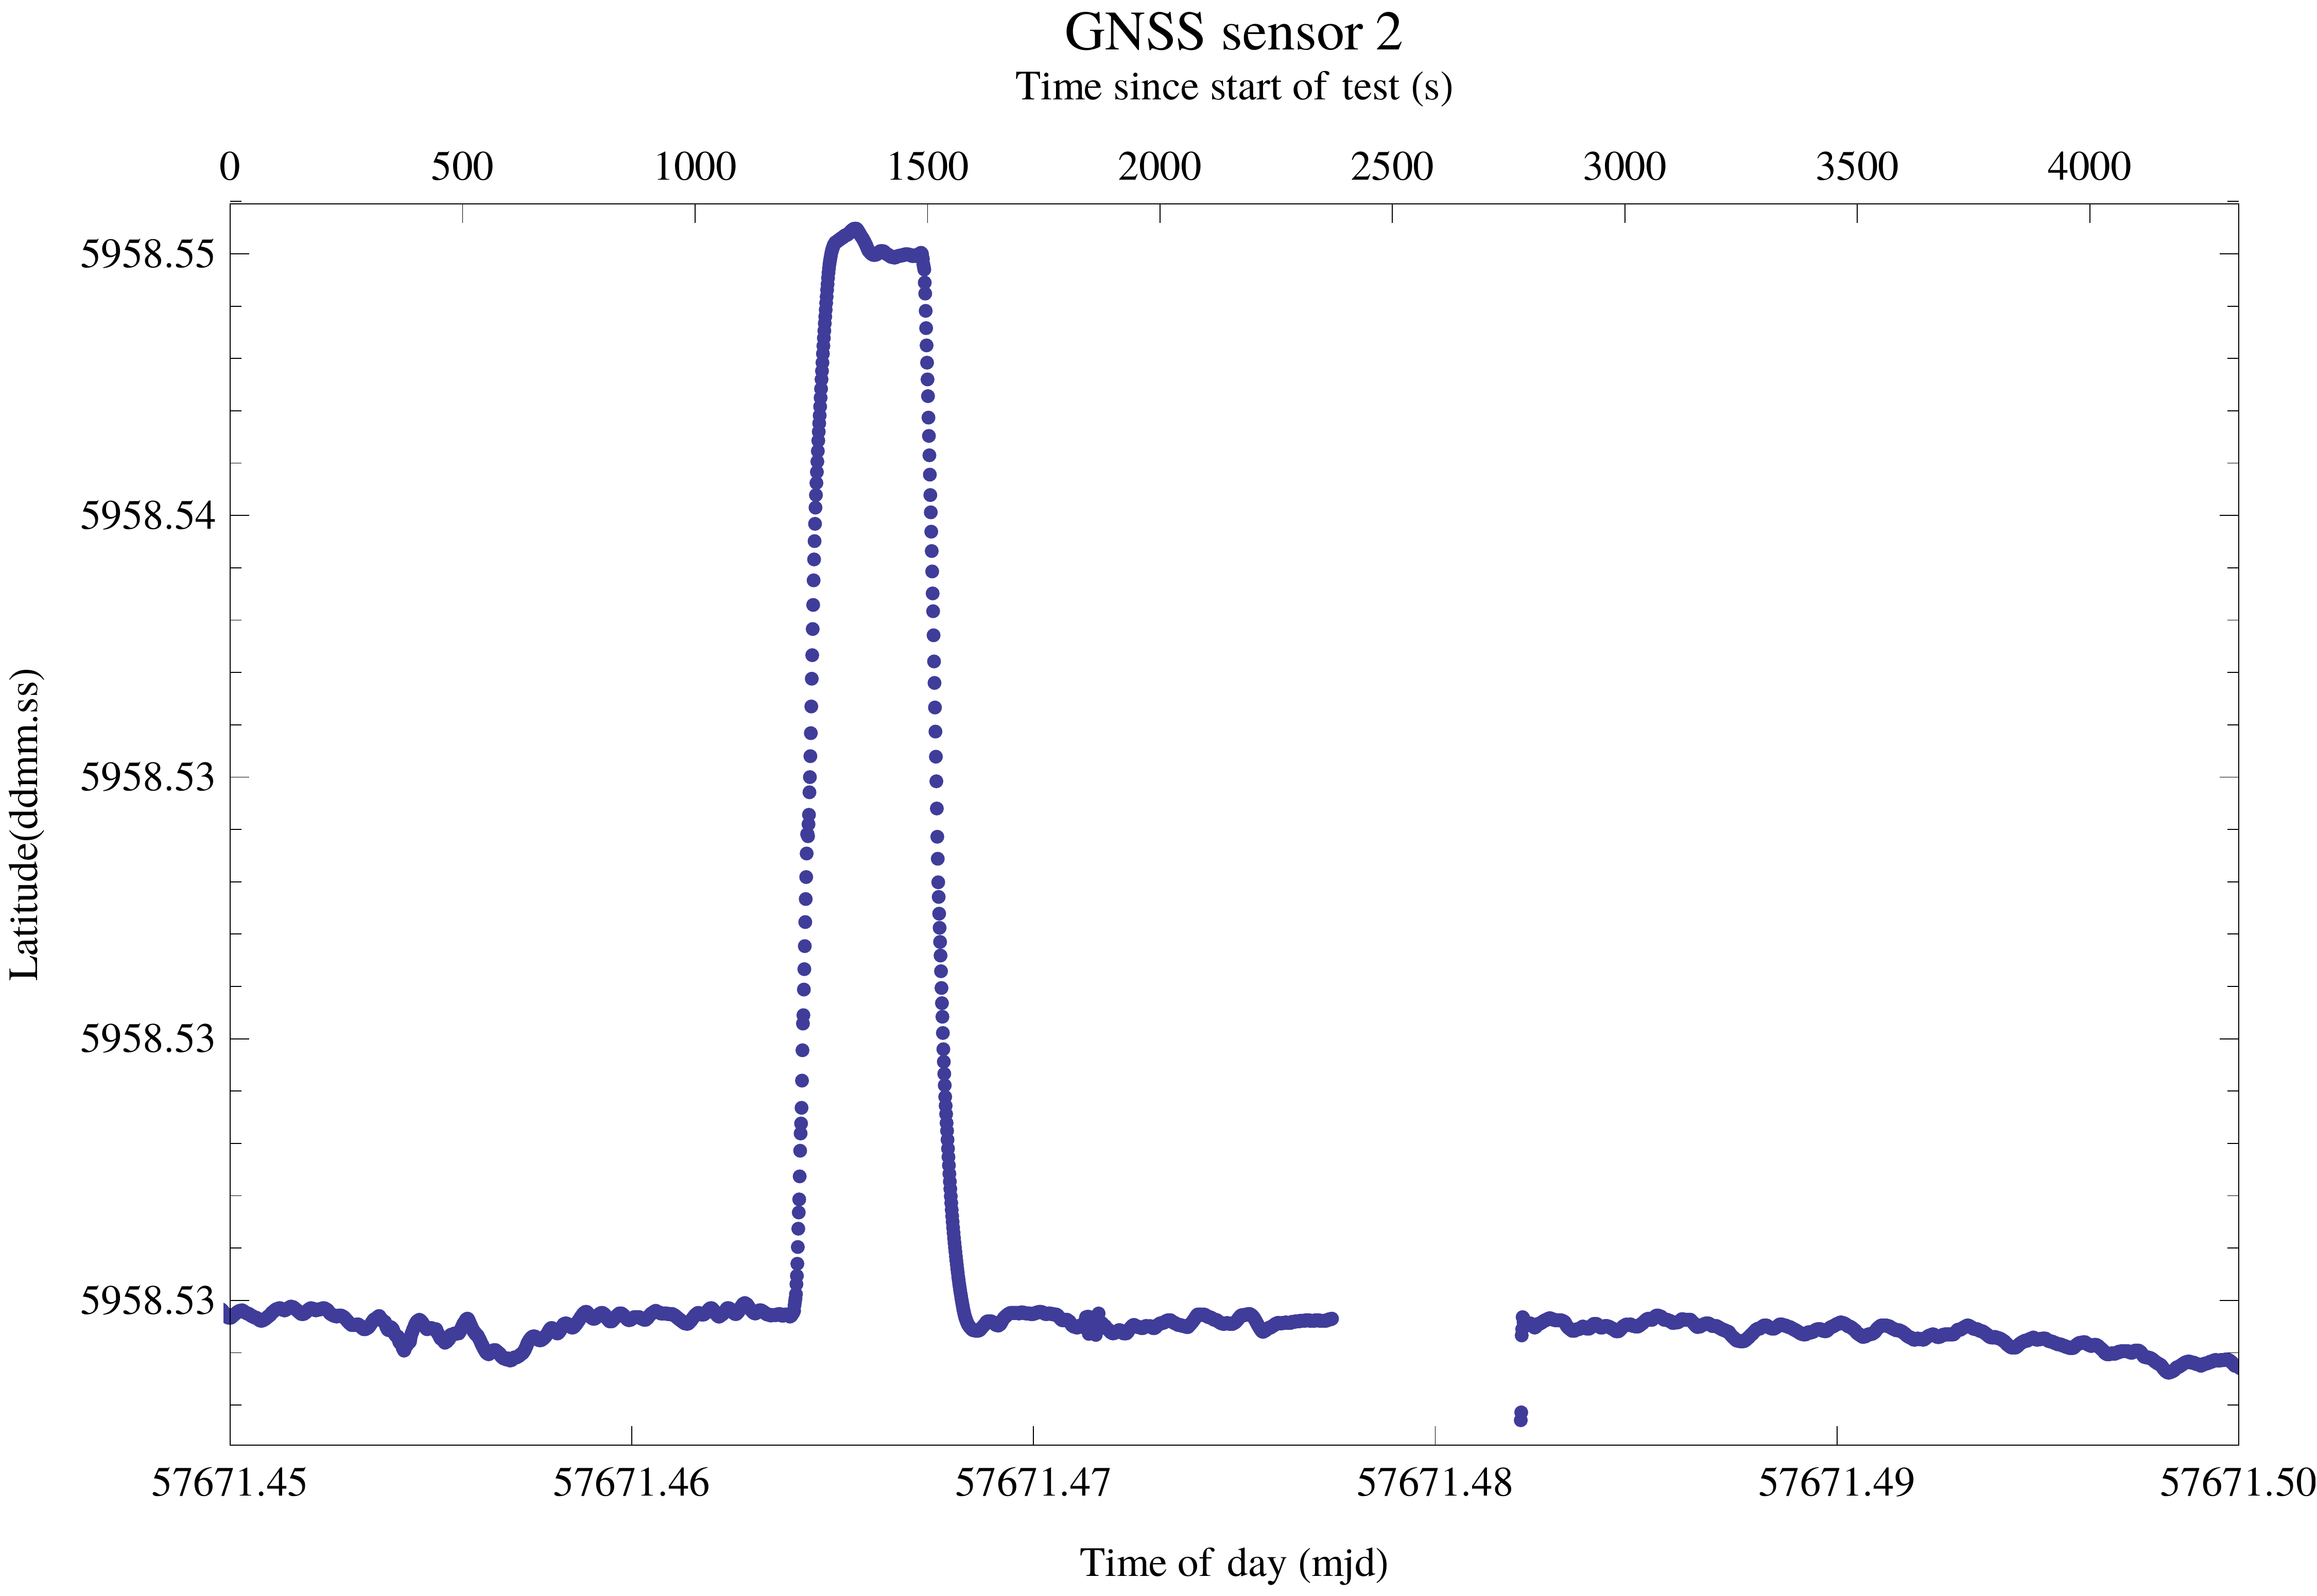
\includegraphics[scale=0.40]{thesis/graphics/gnssLat2-1.png}
      \end{figure}
      \column{0.5\textwidth}
      \begin{figure}
        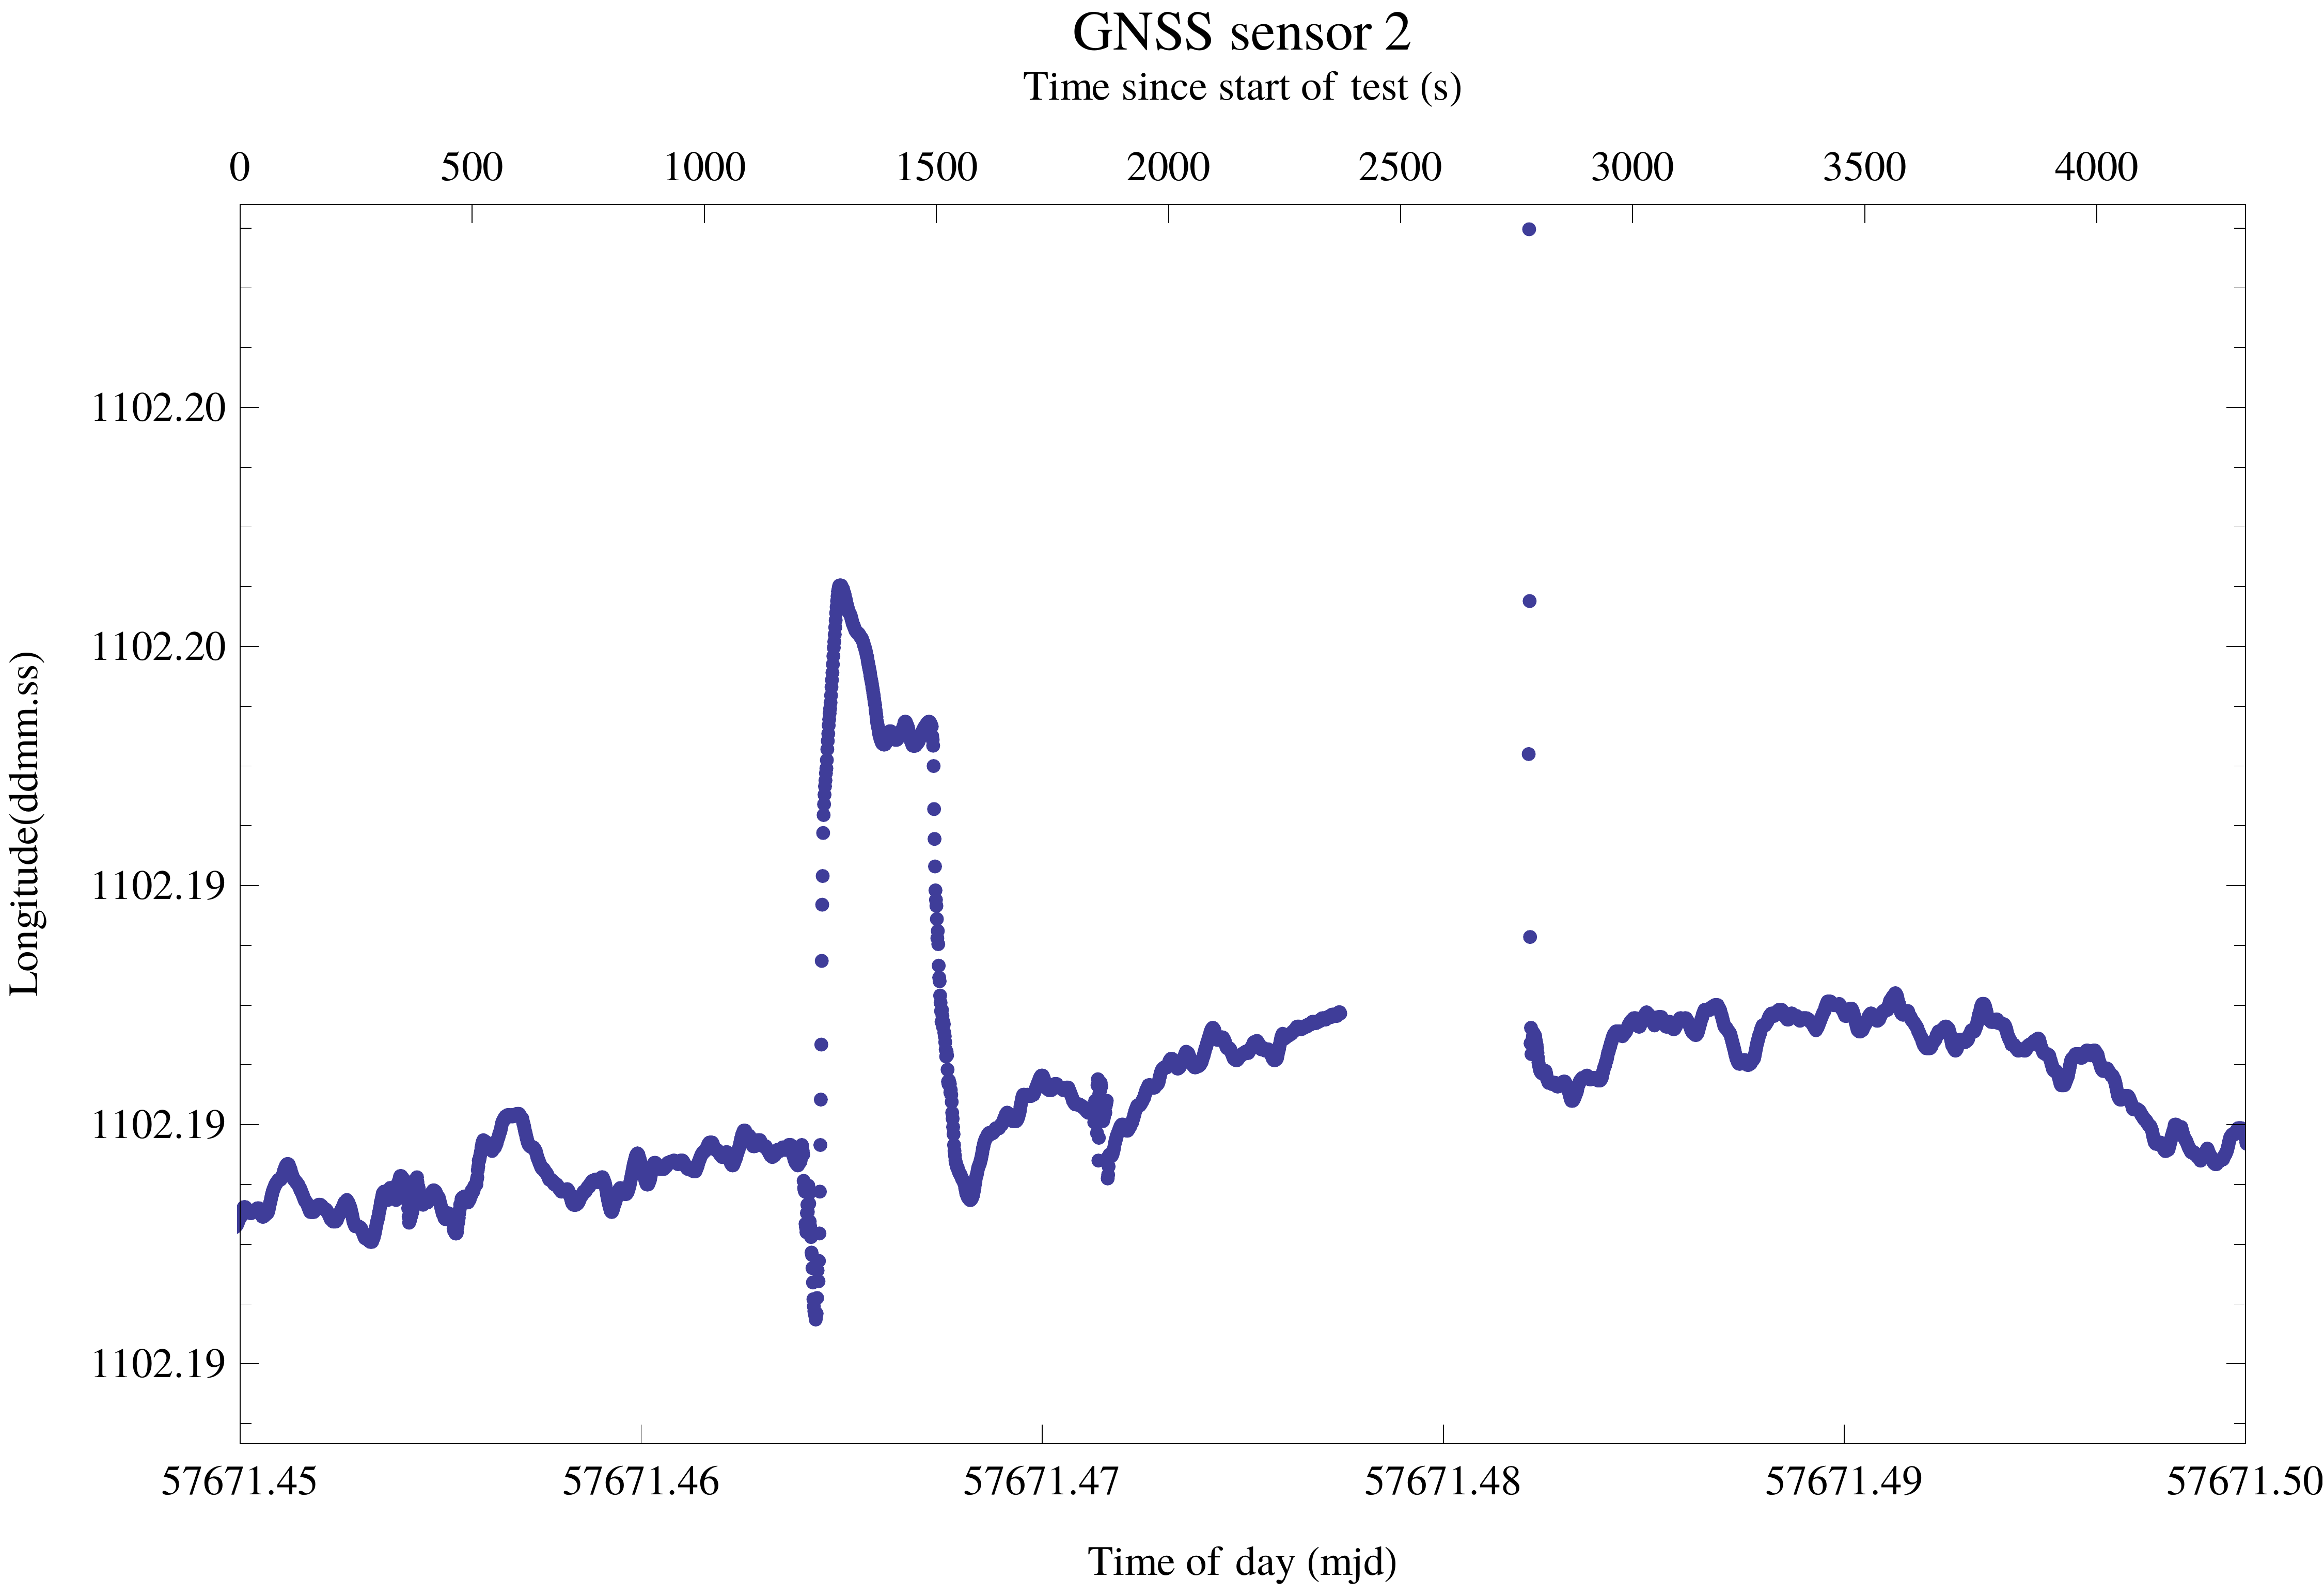
\includegraphics[scale=0.40]{thesis/graphics/gnssLong2-1.png}
      \end{figure}
      \vspace{-30pt}
      \begin{figure}
        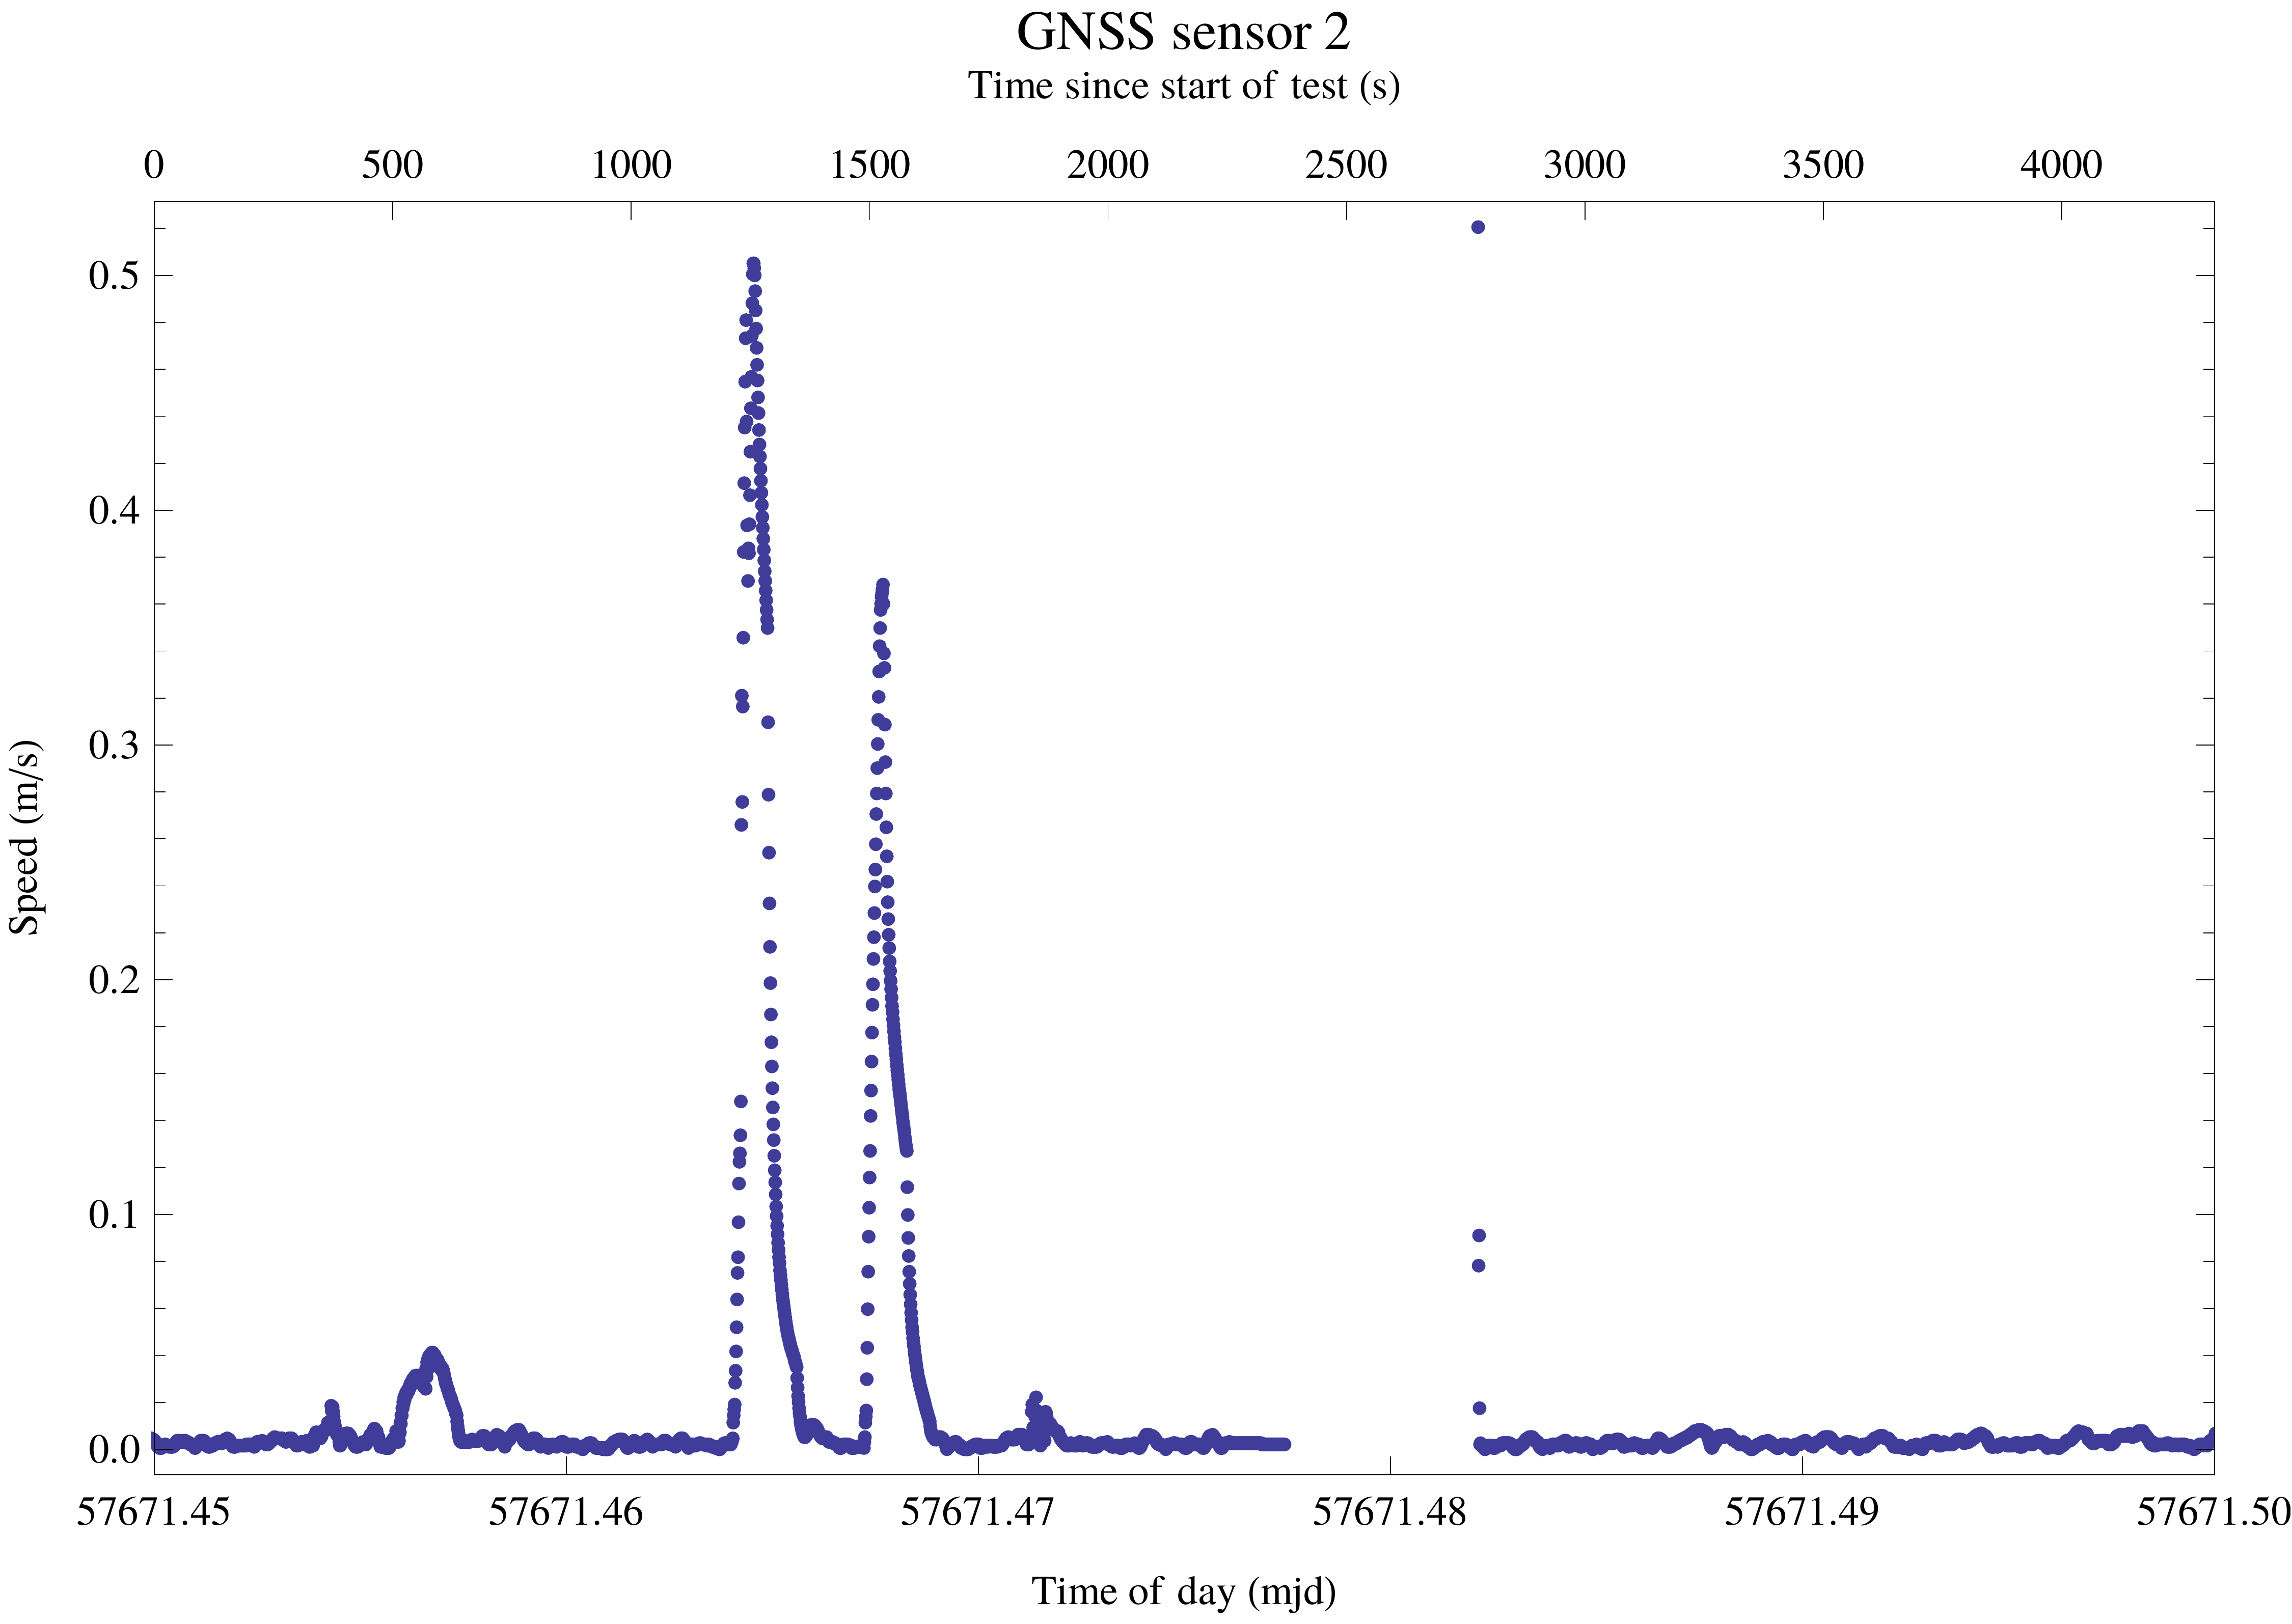
\includegraphics[scale=0.40]{thesis/graphics/gnssSpeed2-1.png}
      \end{figure}
    \end{columns}  
\end{frame}

\begin{frame}
\frametitle{Observasjon: Målesystem}
      \begin{figure}
        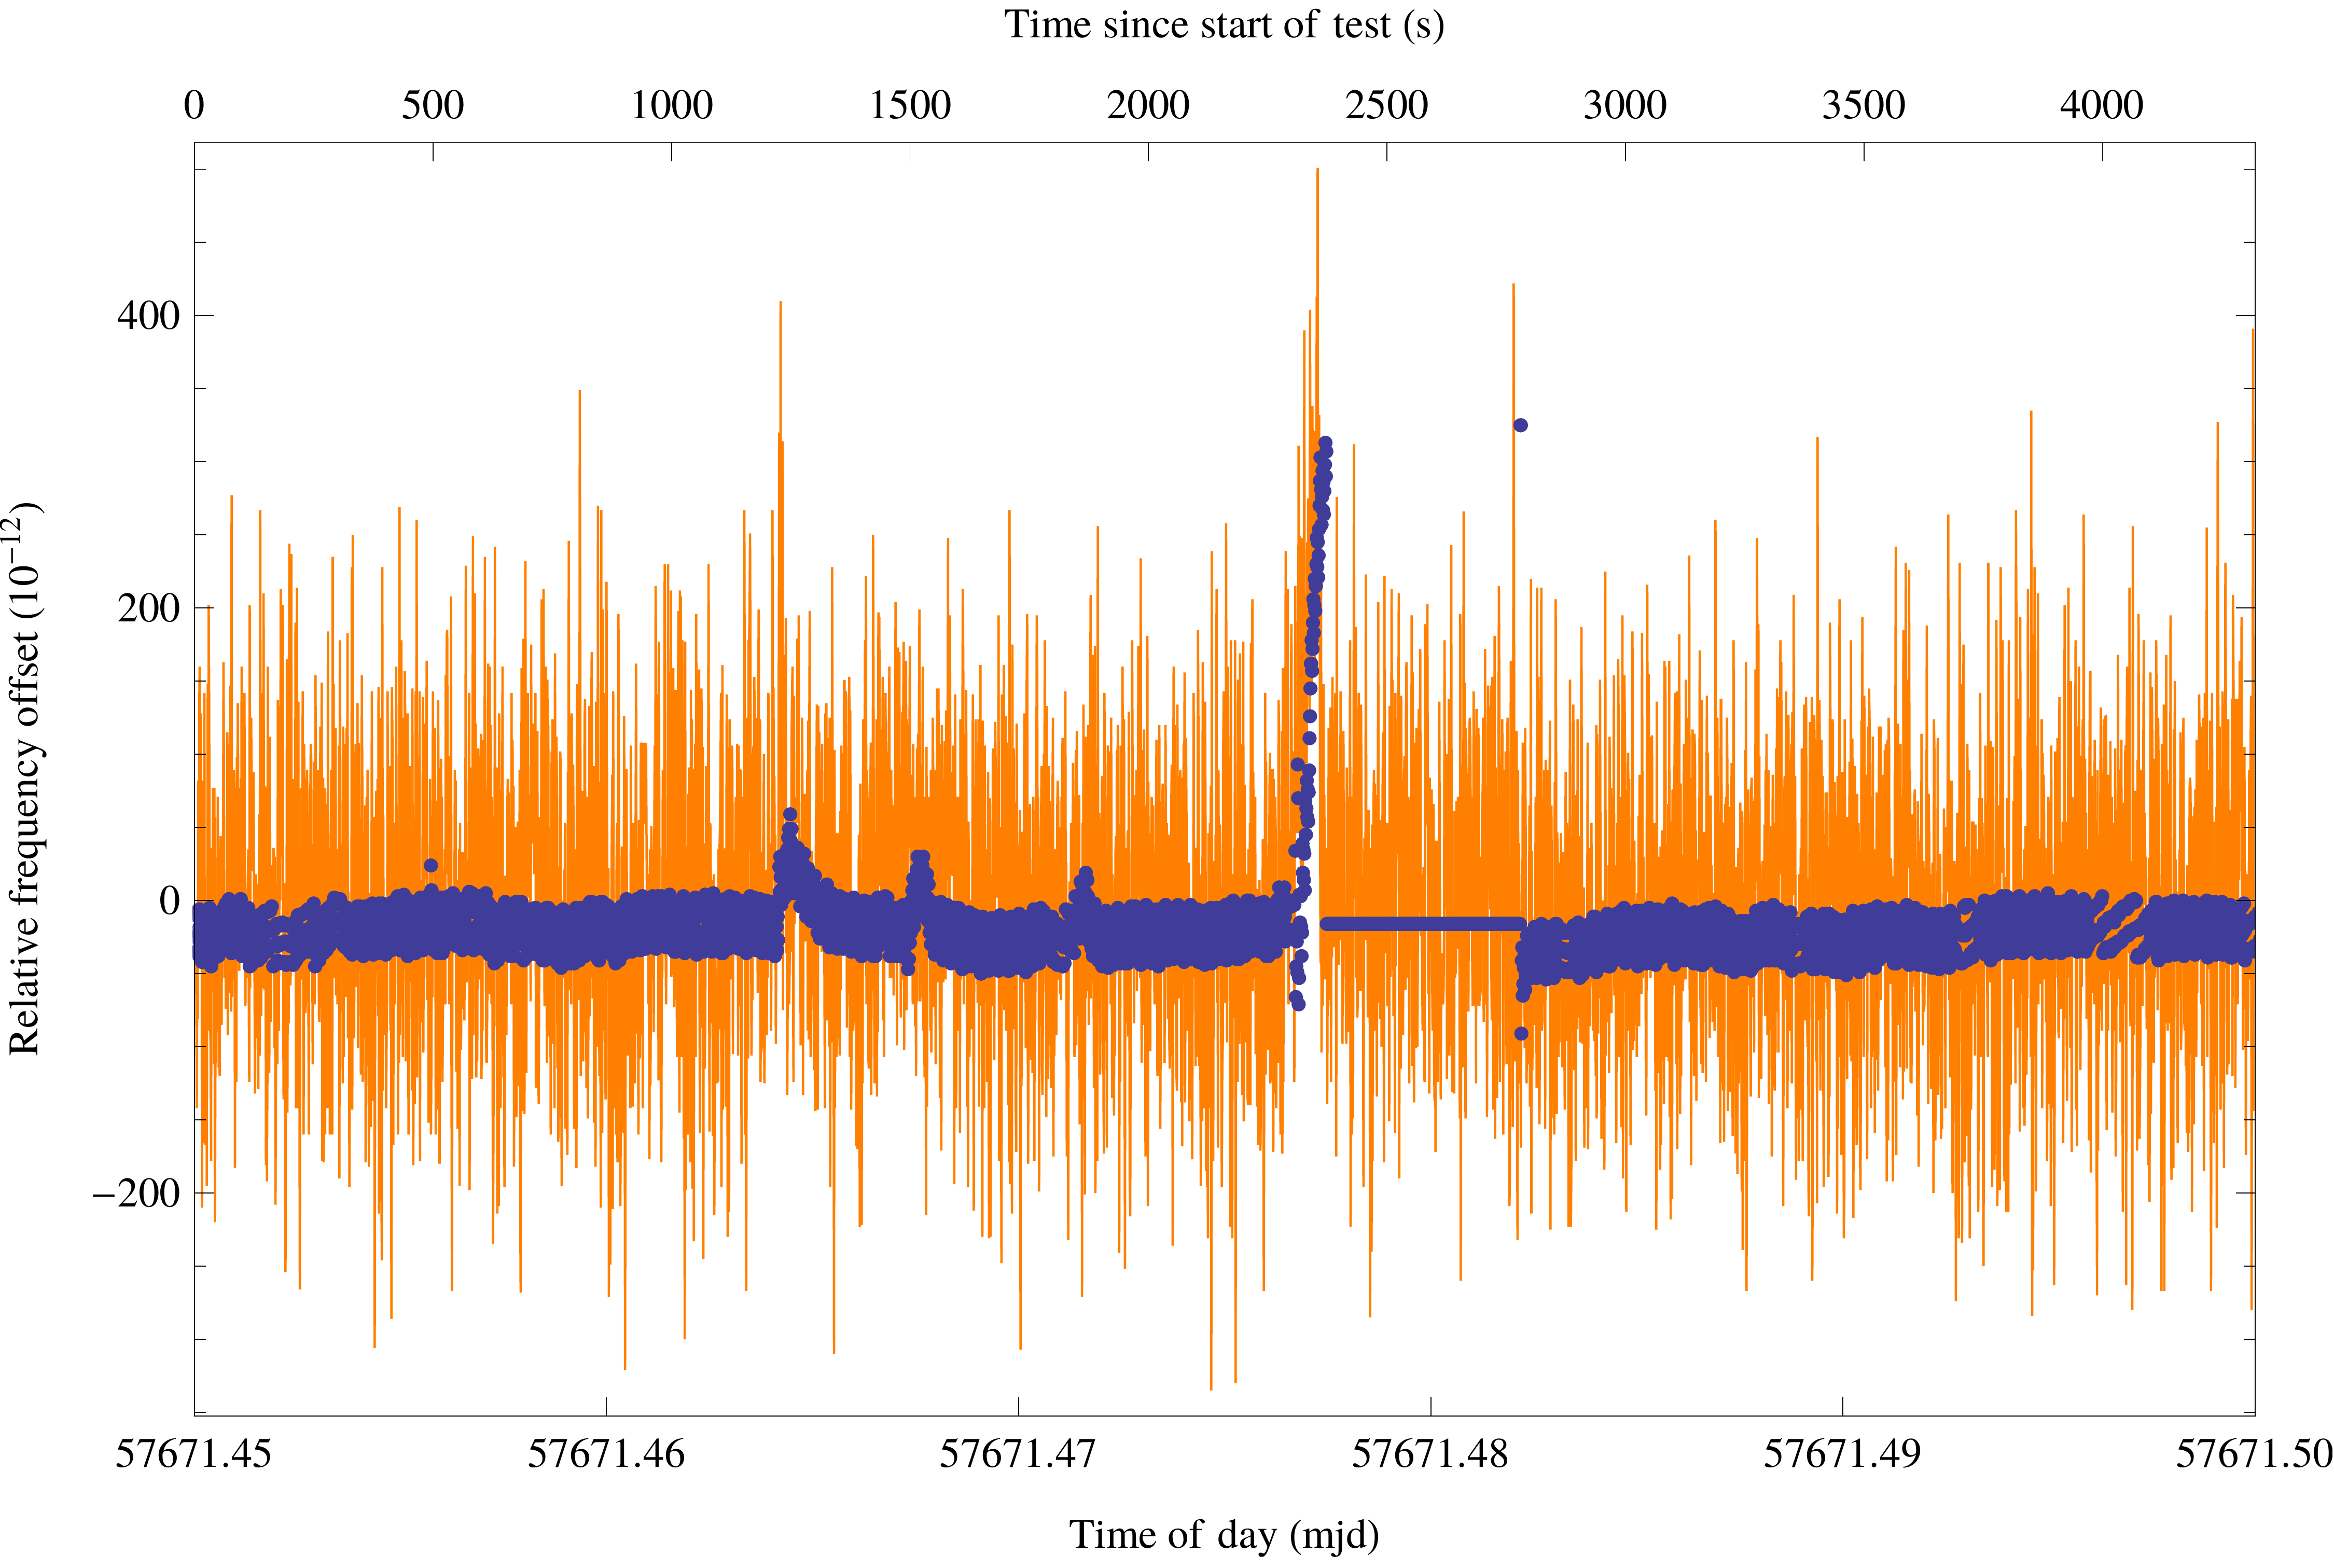
\includegraphics[scale=0.70]{thesis/graphics/cns91-and-csac-telemetry-frequency-1.png}
        \caption{Måleserie gjort under test av lokasjon og hastighetsfilter}
      \end{figure}
\end{frame}

\section{Klokkemodell test}
\begin{frame}
\frametitle{Oppsett}
  \begin{itemize}
    \item Testet klokkemodellen og styring.
    \item Justerte ned grenseverdi for hastighet
    \item Tok bare med en Sensor da fokus var på klokkemodell.
  \end{itemize}
\end{frame}

\subsection{Beskrivelse}
\begin{frame}
  \frametitle{Oppsett: grenseverdier for filter}
    \begin{columns}
    \column{0.5\textwidth}
      \begin{table}[!htb]
      \centering
        \caption{Grenseverdier for lokasjon og hastighetsfilter}
        \label{gps_filter_table2}
          \resizebox{0.9\textwidth}{!}{\begin{tabular}{|l|l|l|}
            \hline
            \multicolumn{1}{|c|}{Config value} & \multicolumn{1}{c|}{Sensor 2} \\ \hline
            Høyde referanse                 & 122.427$^{\circ}$             \\ \hline
            Lengdegrad referanse                & 1102.1934$^{\circ}$           \\ \hline
            Breddegrad referanse                 & 5958.5231$^{\circ}$           \\ \hline
            Hastighet referanse                    & 0 knot                        \\ \hline
            Høyde avvik                 & 10$^{\circ}$                  \\ \hline
            Lengdegrad avvik                & 0.005$^{\circ}$               \\ \hline
            Breddegrad avvik                 & 0.005$^{\circ}$               \\ \hline
            Hastighet avvik                    & 1 knot                             \\ \hline
          \end{tabular}}
      \end{table}

      \column{0.5\textwidth}

      \begin{table}[!htb]
      \centering
      \caption{Klokkemodell konfigurasjon}
      \label{clock_filter_table}
       \resizebox{0.7\textwidth}{!}{\begin{tabular}{|l|l|}
          \hline
          Phase limit      & 50     \\ \hline
          Steer limit      & 50     \\ \hline
          Time constant    & 10000  \\ \hline
          Warmup time      & 2      \\ \hline
          Prediction limit & 200    \\ \hline
        \end{tabular}}
      \end{table}
    \end{columns}
\end{frame}

\begin{frame}
\frametitle{Utførelse}
      \begin{itemize}
        \item 13:12:00 - 125s: Beveget antenne 2 mot nord
        \item 13:23:00 - 785s: Viftet antenne 1 rundt i en halvsirkel
        \item 13:23:45 - 830s: Stoppet bevegelse
        \item 13:27:00 - 1070s: Aktiverte disiplinering av klokka manuelt
      \end{itemize}
\end{frame}

\begin{frame}[fragile]
\frametitle{Observasjon: Server log}
Utdrag fra server log:
    \begin{lstlisting}[basicstyle=\ttfamily\tiny]
      [10/24/16 - 13:12:10] [ ALARM ] Sensor 2 triggered LS filter!
      [10/24/16 - 13:12:42] [ ALARM ] Steer > predicted!
      [10/24/16 - 13:19:54] [ ALARM ] Sensor 2 cleared LS filter!
      [10/24/16 - 13:23:12] [ ALARM ] Sensor 2 triggered LS filter!
      [10/24/16 - 13:23:13] [ ALARM ] Sensor 2 cleared LS filter!
      [10/24/16 - 13:23:15] [ ALARM ] Sensor 2 triggered LS filter!
      [10/24/16 - 13:23:43] [ ALARM ] Sensor 2 cleared LS filter!
    \end{lstlisting} 
\begin{itemize}
  \item Ingen falske positive
  \item Frekvenskorreksjonsfilteret utløst
\end{itemize}
\end{frame}

\begin{frame}
\subsection{Observasjon}
\frametitle{Observasjon: GPS log}
        \begin{figure}
        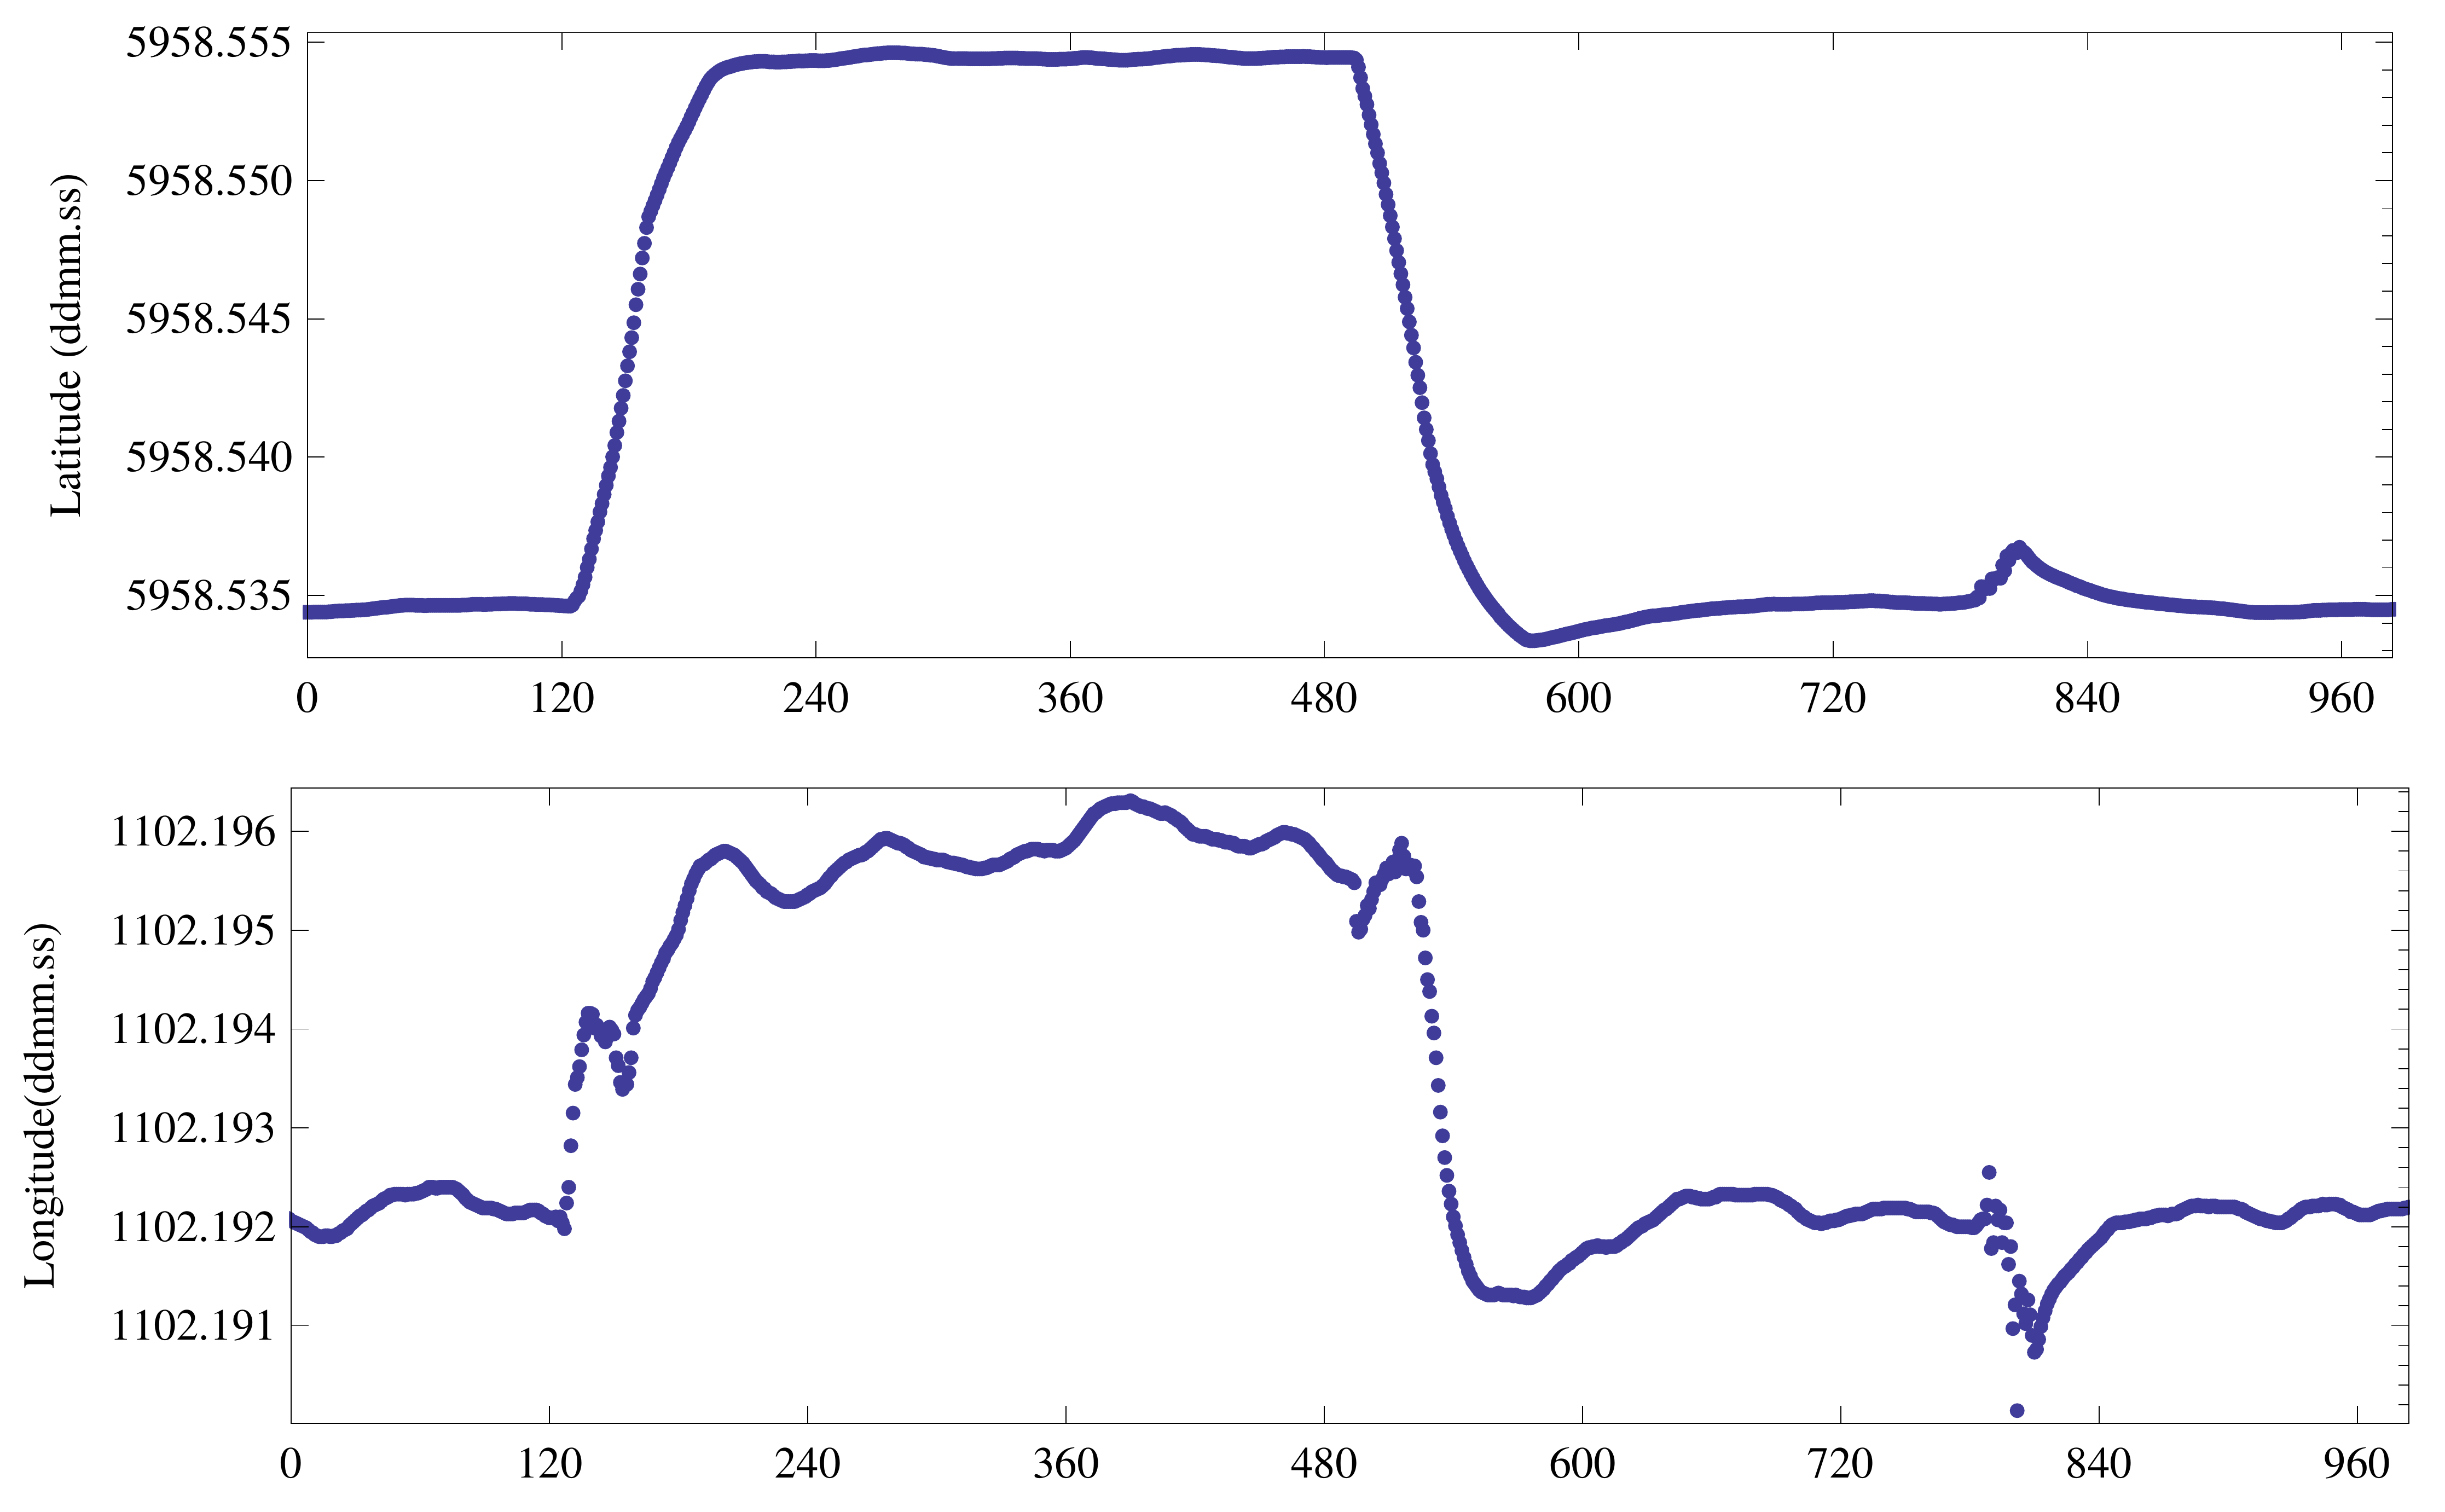
\includegraphics[scale=0.8]{thesis/graphics/20161024-test2-sensor2-multipanel-1-1.png}
        \caption{Lengdegrad og breddegrad}
      \end{figure}
\end{frame}

\begin{frame}
\frametitle{Observasjon: GPS log}
        \begin{figure}
        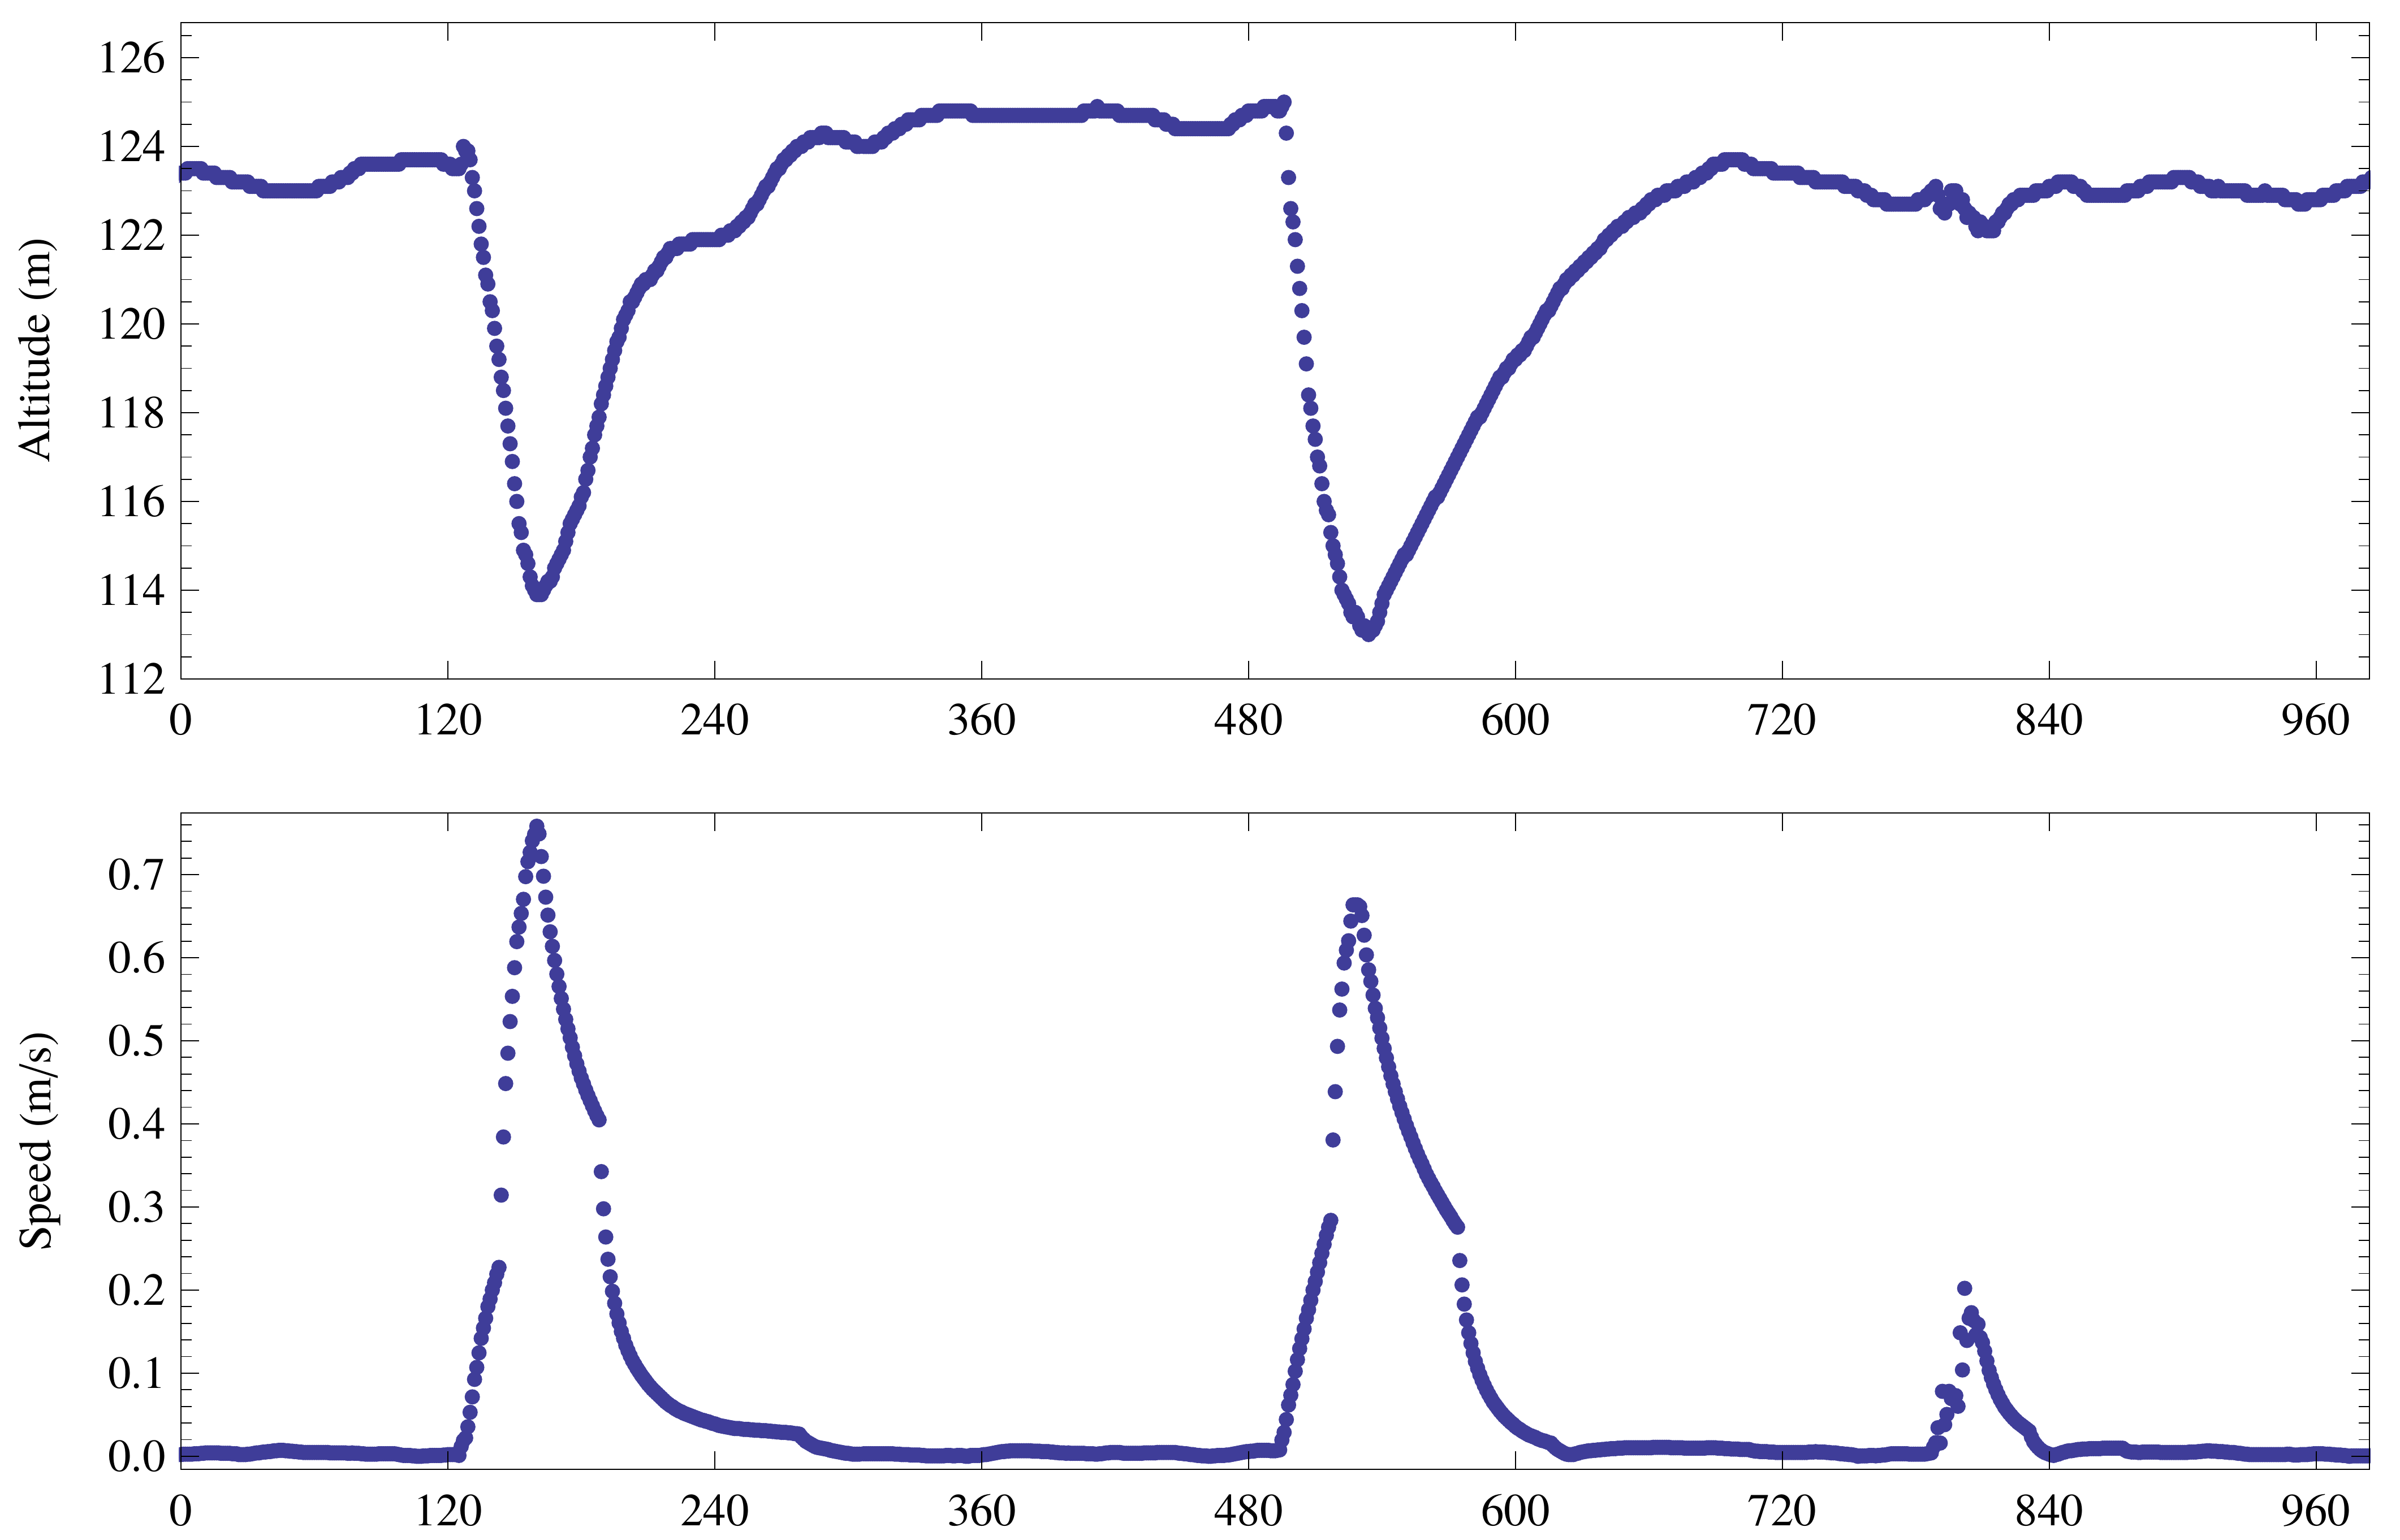
\includegraphics[scale=0.8]{thesis/graphics/20161024-test2-sensor2-multipanel-1-2.png}
        \caption{Høyde og hastighet}
      \end{figure}
\end{frame}

\begin{frame}
\frametitle{Observasjon: Målesystem}
      \begin{figure}
        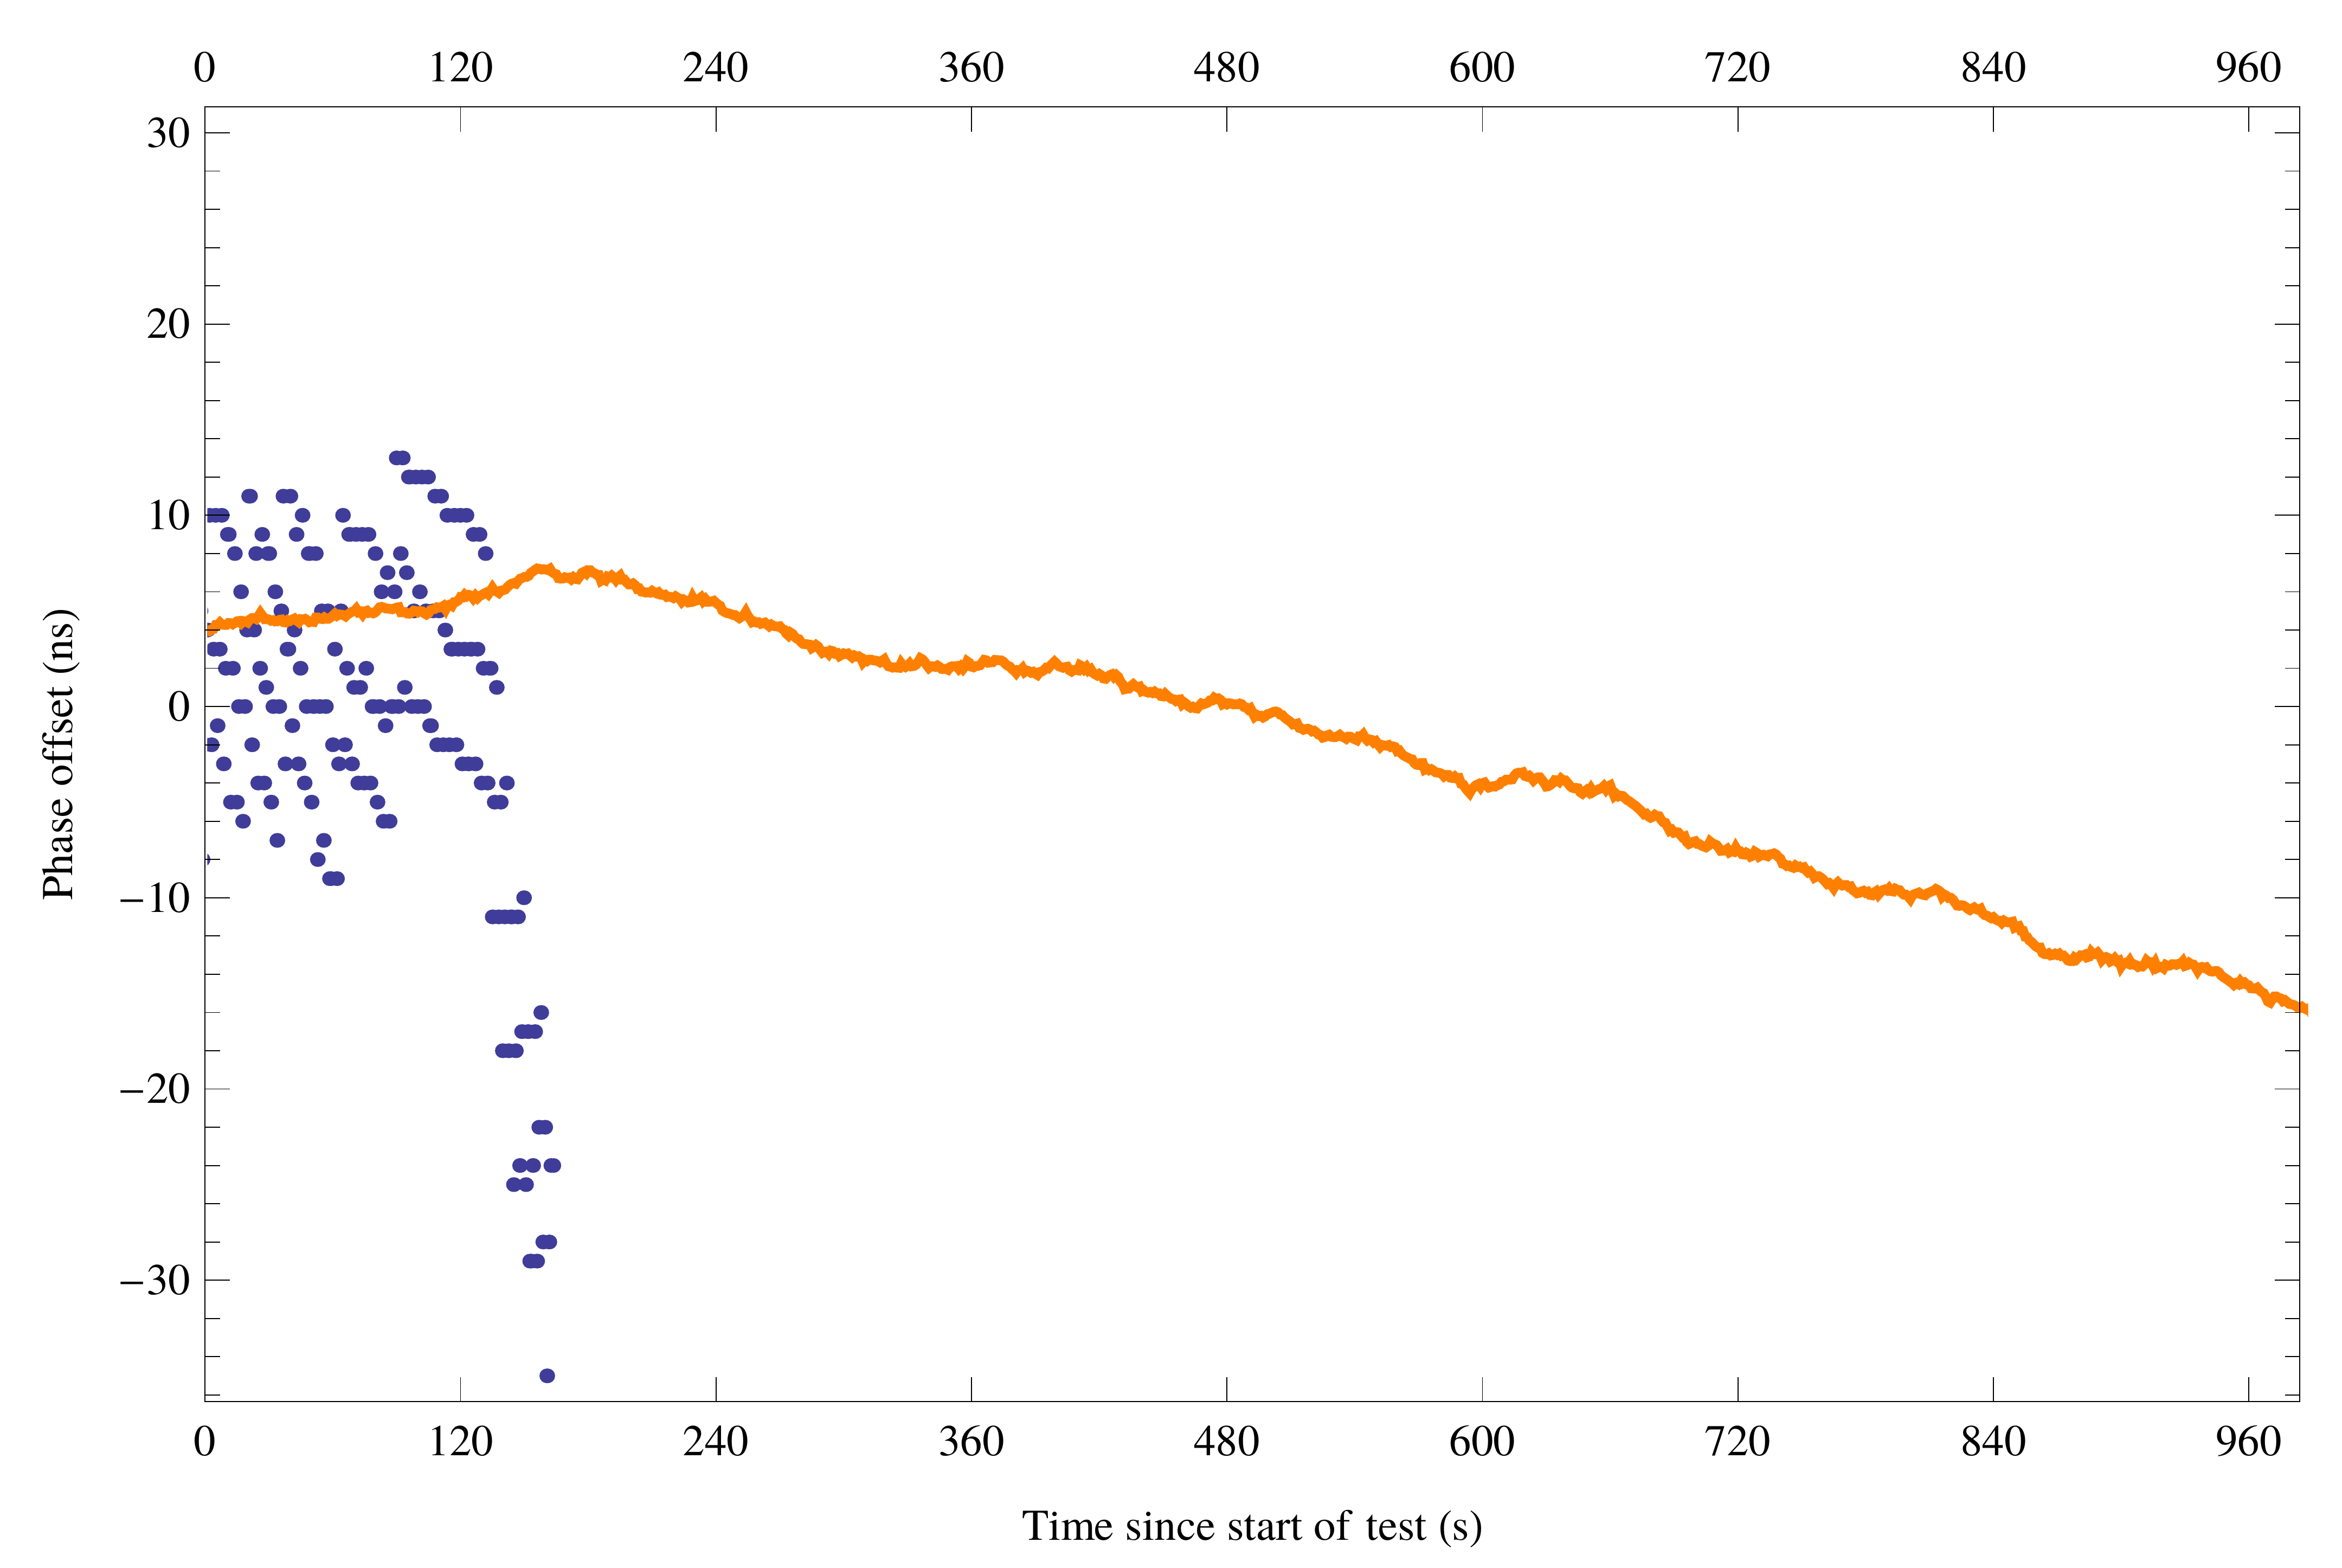
\includegraphics[scale=0.70]{thesis/graphics/20161024-test2-telemetry-and-cnt91-combined-1-1.png}
        \caption{Måleserie gjort under klokkemodell test}
      \end{figure}
\end{frame}

\begin{frame}
\frametitle{Observasjon: Målesystem}
      \begin{figure}
        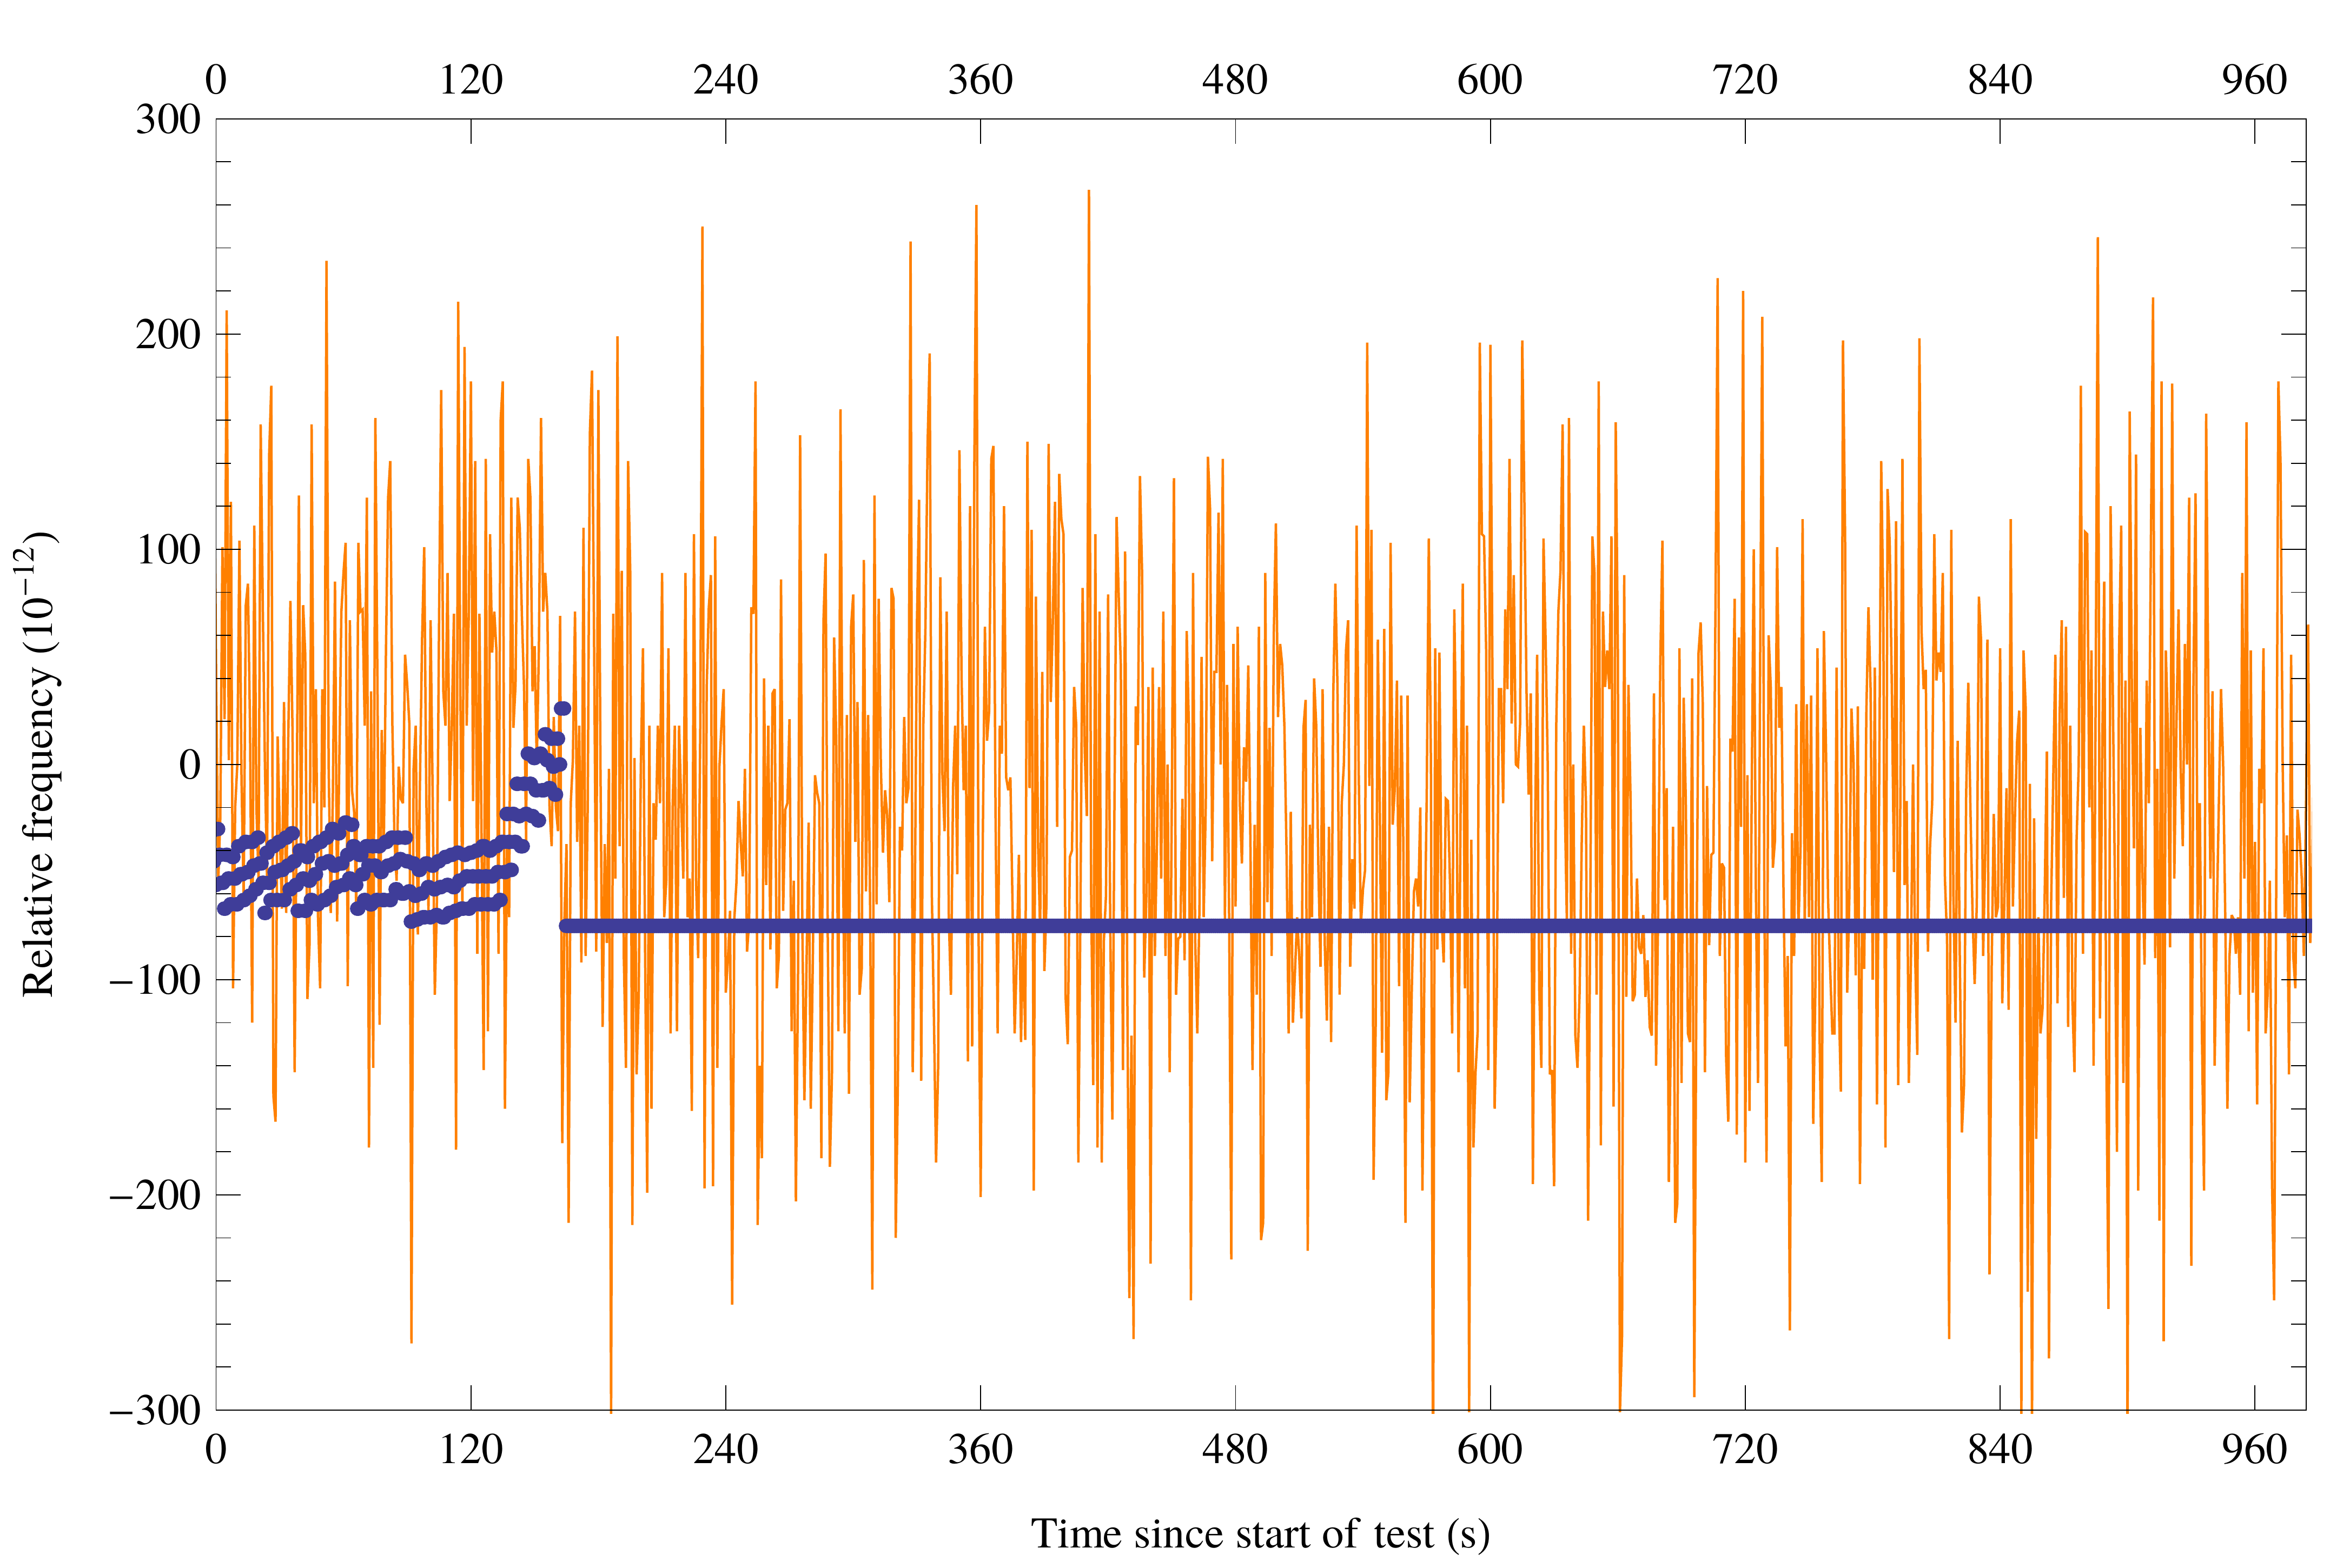
\includegraphics[scale=0.70]{thesis/graphics/20161024-test2-telemetry-and-cnt91-combined-1-2.png}
        \caption{Måleserie gjort under klokkemodell test}
      \end{figure}
\end{frame}

\section{Konklusjon}
\begin{frame}
  \frametitle{Konklusjon}
  Vi har demonstrert:
  \begin{itemize}
    \item At en fullt fungerende \textit{"spoof proof atomic clock controller"} ville ha vært i stand til å stå imot et angrep utført med en sofistikert GPS spoofer slik som \textit{"The Civil GPS spoofer"}.
    \item Nåværende implementasjonen evne til å detektere en forstyrrelse av GPS signaler og en begrenset evne til å begrense skaden av nevnte forstyrrelse.
    \item Effektivitet til Sensor server arkitekturen. 
    \begin{itemize}
      \item Lav responstid
      \item Høy stabilitet 
      \item Enkel å bygge ut med flere sensorer
    \end{itemize}
  \end{itemize}
\end{frame}

\section{I ettertid}
\begin{frame}
  \begin{itemize}
  \item Kommunikasjon med atomklokke
    \frametitle{Ikke løste problemer}
    \begin{itemize}
      \item Antatt å ha vært et problem med konfigurasjonen av serialport.
      \item Systematisk feilsøkt etter innlevering. Forsøkt:
      \begin{itemize}
        \item Forskjellige kabler
        \item Forskjellige datamaskiner
        \item Verifisert med "serial port sniffer", riktig kommando sendes.
      \end{itemize}
      \item Kan være et fastvare problem
    \end{itemize}
  \item GPS filter ikke ferdig integrert.
  \end{itemize}
\end{frame}

\section{Bibliografi}
\begin{frame}[allowframebreaks]%in case more than 1 slide needed
  \frametitle{Bibliografi}
  \printbibliography[heading=bibintoc]
\end{frame}

\end{document}